\documentclass[11pt,a4paper]{article}
\usepackage{fontspec}
\setmainfont[Path=../tmp/pdf_fonts/,BoldFont=NotoSerifCJKsc-Regular.otf,BoldFeatures={FakeBold=2},ItalicFont=NotoSerifCJKsc-Regular.otf,ItalicFeatures={FakeSlant=0.15}]{NotoSerifCJKsc-Regular.otf}
\setsansfont[Path=../tmp/pdf_fonts/,BoldFont=NotoSerifCJKsc-Regular.otf,BoldFeatures={FakeBold=2},ItalicFont=NotoSerifCJKsc-Regular.otf,ItalicFeatures={FakeSlant=0.15}]{NotoSerifCJKsc-Regular.otf}
\setmonofont{DejaVu Sans Mono}[Scale=0.86]
\XeTeXlinebreaklocale "zh"
\XeTeXlinebreakskip=0pt plus 1pt
\usepackage[margin=23mm,headheight=15pt]{geometry}
\usepackage{amsmath,amssymb,amsthm,mathtools,bm}
\usepackage{graphicx,booktabs,longtable,array,tabularx,enumitem,xcolor}
\usepackage{needspace}
\usepackage[unicode,colorlinks=true,linkcolor=black,citecolor=black,urlcolor=blue!45!black,breaklinks=true]{hyperref}
\usepackage{fancyhdr}
\pagestyle{fancy}\fancyhf{}\fancyhead[L]{\small Research Z-ALG}\fancyhead[R]{\small 材料等价结构与概率纤维}\fancyfoot[C]{\thepage}
\renewcommand{\headrulewidth}{0pt}
\setlength{\parindent}{0pt}\setlength{\parskip}{5pt}
\linespread{1.14}
\setlist{nosep,leftmargin=1.7em,topsep=4pt,itemsep=3pt}
\setlength{\emergencystretch}{2em}
\allowdisplaybreaks[2]
\newtheorem{proposition}{命题}[section]
\newtheorem{theorem}[proposition]{定理}
\newtheorem{corollary}[proposition]{推论}
\theoremstyle{definition}\newtheorem{example}[proposition]{例}
\newtheorem{remark}[proposition]{说明}
\renewcommand{\proofname}{证明}
\renewcommand{\contentsname}{目录}
\renewcommand{\figurename}{图}
\newcommand{\M}{\mathcal M}\newcommand{\Z}{\mathcal Z}\newcommand{\Y}{\mathcal Y}\newcommand{\U}{\mathcal U}
\newcommand{\F}{{\mathcal F_a}}\newcommand{\rank}{\operatorname{rank}}\newcommand{\im}{\operatorname{im}}
\newcommand{\diag}{\operatorname{diag}}\newcommand{\TV}{\operatorname{TV}}\newcommand{\E}{\mathbb E}
\newcommand{\R}{\mathbb R}\newcommand{\C}{\mathbb C}\newcommand{\supp}{\operatorname{supp}}
\newcommand{\norm}[1]{\left\lVert #1\right\rVert}\newcommand{\Hh}{\mathcal H}
\newcommand{\tagstd}{\textbf{资格：标准数学及其直接推论。}}
\newcommand{\tagphy}{\textbf{资格：本报告给出的 Maxwell 条件推导，不作数学首创声明。}}
\newcommand{\tagnumer}{\textbf{资格：本轮实际完成的小型数值验证。}}
\hypersetup{pdftitle={Research Z-ALG Maxwell材料等价结构与概率纤维},pdfauthor={Research Z-ALG},pdfsubject={严格数学框架、Maxwell专化、分支覆盖、条件测度与最小实验协议}}
\begin{document}
\pagenumbering{gobble}
\begin{titlepage}
\vspace*{18mm}
{\LARGE\bfseries Research Z-ALG\par}
\vspace{10mm}
{\huge\bfseries Maxwell 材料等价结构\par}
\vspace{4mm}
{\huge\bfseries 可观测商与概率纤维\par}
\vspace{12mm}
{\large 从多表示的合法对应到精确分支生成与正确条件测度\par}
\vspace{12mm}
{\large 中文理论科研报告\par}
{\normalsize 2026 年 10 月 29 日\par}
\vspace{12mm}
\textbf{主判断}\quad 值得建立独立的 Research Z-ALG，但研究主轴应是可验证的材料等价关系、限定域分支覆盖与条件概率积分。一般 Maxwell 观测纤维不必是简单群的轨道；群胚的存在也不会自动给出可计算生成元。

\textbf{优先架构}\quad 用精确接收约束参数化同观测电流，再用多照明共享材料的代数约束恢复合法材料；在有证据的对称分支上复用物理计算，在其余分支上保留明确的覆盖资格，最终从原材料先验构造条件核。

\textbf{本轮实质结果}\quad 给出严格条件定理和反例，完成二单元 Hankel-Green TM/VIE 的离散交换等价、商反演和暗电流反例，核验解析 toy 的复 monodromy。上述小型见证不构成 Full66 全后验恢复或一般 Maxwell 全解枚举的证据。
\vfill
\small 物理材料、表示冗余、观测等价、有限噪声相容及后验质量分别定义。所有新算法与大规模外推均有独立的适用条件。
\end{titlepage}
\pagenumbering{roman}
\tableofcontents
\newpage
\pagenumbering{arabic}
\section{研究判断与证据边界}

\subsection{五个直接结论}

本研究的总体答案是\textbf{有条件地肯定}。Maxwell 多解可以比一组无关联的优化终点更有结构，但不存在一套对所有材料类、所有采集和所有先验都适用的简单群。真正可用的结构应满足四个条件：连接的是不同合法材料；保持完整带标签观测；能以较低费用生成或验证；能保留原先验的条件质量。

第一，\textbf{精确有限对称确实可以产生不同材料的离散等价分支}。本轮二单元 TM/VIE 例子中，交换两个镜像位置的材料保持全部复观测。可先反演两个对称不变量，再用二次方程列出该材料族中的全部两支。两个分支附近的材料响应都满秩，所以它没有连续精确 null 方向。局部满秩与远处多解可以同时成立。

第二，\textbf{更宽材料类中的正维精确纤维也有严格成立的条件}。原 Full66 的八个重建中心不满足这一前提；完整的 $24\times24$ 固定复相位材料类则具有 576 个实自由度，而 $8\times32$ 个复观测最多为 512 个实坐标。在合法内点且常秩 $r$ 的区域，精确纤维维数是 $576-r\ge64$。这改变了 prior/support，不能回写成原 Full66 的结果。

第三，\textbf{多数材料等价关系更适合用受约束纤维、分支图册与对应关系组织}。关系群胚可以准确记账，却不会自动给出生成元；有群作用也只说明轨道包含在纤维内，不说明覆盖全部逆解。正维连续纤维不能由有限个固定变换的有限字词逐点列完。

第四，\textbf{无损商反演的关键是 likelihood 因子化和可计算的条件核}。若 $\F=h\circ\pi$，且 $K(dm\mid u)$ 是原材料 prior 的条件分布，则只反演 $u$ 后可精确恢复材料后验。写出这个分解不保证计算变简单；有限群商通常不降低连续维数，条件权重也可能很难算。

第五，\textbf{最值得先做的架构是共享材料约束的电流纤维图册}。先精确满足接收方程，再以多照明共享材料的二次约束排除假电流，并针对场节点、材料支持和 resolvent 给出完整条件。已证明的物理对称可免去重复 Maxwell 求解；其他关系必须继续支付校正、分支发现或认证费用。

\subsection{历史证据如何进入本报告}

已核查 R6 指定科学版本的主报告、理论、分层概率和 copula 控制；R7 主报告、Full66 gauge 审计、E2、理论、费用及 Go/No-Go；旧 Research Z 的主报告、理论与 claim ledger；SOM/TSOM 原作者综述。R6/R7 原始大实验未在本轮重跑，下面把文档核验与本轮新增小型计算分别标识。[I1--I4]

\begin{longtable}{p{.18\textwidth}p{.38\textwidth}p{.36\textwidth}}
\toprule
证据 & 保留的结论 & 对 Z-ALG 的约束\\\midrule\endhead
R6 同材料纤维 & 固定 $V=QD$ 的联合配对给相同材料；保持经验边缘却打乱依赖，Full 响应白化控制距离均值约 15.526 与 117.578。 & 属 decoder gauge 与条件依赖反例；不是新材料 Maxwell nullspace，也不是完整 posterior 样本。\\
R6 分层概率 & host、transition、pure 源层及材料像重叠须分开；局部积分收敛不能证明远分支和尾部已覆盖。 & 不能把单点 Jacobian 为零等同于全局任务对数据不响应；不能用 prior 归一化合格代替 posterior 资格。\\
R7 Full66 & 四个特定无 pure-cell 点存在数值同材料路径，最大材料 RMS 约 $2.42\times10^{-16}$；另有无 pure 点不满足同样降维。 & gauge 是分层和局部的，不存在已证明的通用一维尺度商。数值秩依赖阈值。\\
R7 八个新对象 & 普通动态 Full-J 均找到 $0.02$ 材料 RMS 的竞争端点，其中七例另满足成对距离不超过 1；八中心材料有效响应数值秩均为 66。 & 有限噪声歧义成立；精确连续材料纤维未建立；局部满秩不排除远处离散多解。\\
R7 高阶路线 & Jets 当前实现未胜普通 Full-J；实现范围和接缝限制均保留。 & 不将高阶反馈重新命名为群生成元；也不把实现 No-Go 当作所有高阶理论的否定。\\
F/F3 与旧 Z & 局部候选和若干补偿并未建立跨拓扑全解覆盖；旧 Z 是 2026-10-15 理论设计包，无新训练或 Maxwell 后验样本。 & 新正面见证必须独立建立；扩大材料类须明确新 prior，不能改写原 P0 结果。\\
SOM/TSOM & 确定电流与模糊电流分解、内部传播相关子空间、Fourier 加速已有成熟前例。 & current relevance、材料可实现性、材料可辨识性与任务风险必须分开。\\\bottomrule
\end{longtable}

特别是 R6 的 ``均匀 $V=QD$'' 指的是所考察的均匀材料子模型，\emph{并不表示条件 prior 自动均匀}。其复属性到材料的条件 Jacobian 含 $Q^2$，正确纤维权重包含 $Q^{-2}$。后文另给的简单双曲线 toy 使用显式指定的新 prior，不能替代 R6 原先验。

\subsection{结果资格}

\textbf{标准数学}包括常秩定理、逆函数定理、轨道与群胚、覆盖空间、coarea、disintegration、MH 和已有数值代数几何。

\textbf{Maxwell 条件推导}包括固定标签的交换条件、共享材料 minors 的等价条件、残差到真实数据的 resolvent 证书，以及二单元商恢复公式。本文给出证明，但不把这些标准工具的组合自动宣布为文献首创。

\textbf{本轮实际计算}包括二单元离散 VIE、真实 Green 圆盘积分复核、暗电流反例、解析 Jacobian 对照、三次多项式 monodromy 与若干低维积分公式。它们支持本报告所标明的有限范围。

\textbf{待验证研究主张}是非对称小型 Maxwell 系统中的更完整分支发现、更便宜的任务积分、全 prior 质量恢复及跨 decoder 的独立费用收益。后续实验协议不把这些主张预写为成功。

\section{统一的材料与多 Decoder 框架}

\subsection{先固定物理与统计合同}

将所有复变量视为实向量空间，避免把复自由度和实自由度混算。一次采集 $a$ 包括频率、源场、接收位置与极化、标签、背景、离散化和噪声约定。合法材料集合 $\M$ 同时包含被动性、几何范围、构成关系、边界条件和本次声明的 prior 支持。不同支持集对应不同反问题。

设材料先验为概率测度 $\mu_0$，已知噪声协方差为 $\Gamma_a\succ0$，取 $W_a^\top W_a=\Gamma_a^{-1}$。观测模型为
\begin{equation}
M\sim\mu_0,\qquad Y=\F(M)+\eta,\qquad
L_y(m)=\exp\left[-\tfrac12\norm{W_a(\F(m)-y)}^2\right].
\end{equation}
对原复 circular Gaussian 数据，实化时的 $\sqrt2/\sigma$ 约定必须与历史合同一致。若噪声协方差、源增益或校准也依赖未知量，应将相应变量加入模型，不能继续把均值 $\F(m)$ 的相等当作整个 likelihood 家族相等。

在唯一、稳定的前向求解域内，$\F$ 是单值映射。若宣称包括非唯一的 Maxwell 边值问题，必须先定义物理解选择或联合状态关系，不能使用没有定义的单值 resolvent。

\subsection{单值 Decoder 与关系 Decoder}

对单值 $G_i:\Z_i\to\M$，可直接定义 $H_i=\F\circ G_i$。对关系
\begin{equation}
\mathcal D_i\subset\Z_i\times\M,
\end{equation}
必须保留潜变量和材料的\textbf{关联状态}：
\begin{equation}
\mathcal E_i=\{(z,m):(z,m)\in\mathcal D_i\},\qquad
\mathcal E=\bigsqcup_i\mathcal E_i,\qquad p(i,z,m)=m.
\end{equation}
然后研究 $\mathcal E\xrightarrow{p}\M_{\rm cov}\xrightarrow{\F}\Y_a$，其中 $\M_{\rm cov}=p(\mathcal E)$ 只是这些表示实际覆盖的材料。

\begin{example}[共享某个原像不构成 latent 等价]
若 $\mathcal D(z_1)=\{a\}$、$\mathcal D(z_2)=\{a,b\}$、$\mathcal D(z_3)=\{b\}$，则前两者及后两者各有共同材料，但 $z_1,z_3$ 没有。故 ``存在某个共同材料'' 不传递。引入 $(z,m)$ 后，这一漏洞消失。
\end{example}

仅给 $z$ 的 prior 和一个多值关系也不足以定义材料 prior。还需给 $m\mid z$ 的选择核，或直接给 $\mathcal E_i$ 上的概率测度；否则不同关系分支的概率根本尚未定义。

\subsection{三种关系及任务层}

在 $\mathcal E$ 上定义
\begin{align}
\mathcal R_G&=\mathcal E\times_{\M}\mathcal E,\\
\mathcal R_{\rm obs}&=\mathcal E\times_{\Y_a}\mathcal E.
\end{align}
前者记录同材料重复表示，后者允许不同材料但相同观测。先识别 $\mathcal R_G$，再判断 $\mathcal R_{\rm obs}$ 的箭头是否真正改变材料。对单值 decoder，得到用户提出的 $z_i\sim_Gz_j$。

材料层的精确关系为 $m\sim_{\F}m'\iff\F(m)=\F(m')$。相应集合商 $\M/\!\sim_\F$ 总是存在，但其拓扑未必是一张流形；若直接取 $\U=\Y_a$ 和 $\pi=\F$，测度论上最稳妥，然而没有获得降维或免费生成能力。

有限噪声距离
\begin{equation}
d_a(m,m')=\norm{W_a(\F(m)-\F(m'))}
\end{equation}
是材料上的伪距离：不同材料可有距离零。阈值关系 $d_a\le\epsilon$ 一般不传递。例如 $F(x)=x$，三点 $0,0.75\epsilon,1.5\epsilon$ 两两相邻成链，首尾却不相容。因此其连通分量不能作为精确等价类。

给定任务 $\psi:\M\to\R^k$，可定义纤维振幅
\begin{equation}
\operatorname{osc}_\psi(u)
=\sup_{m,m'\in\pi^{-1}(u)}\norm{\psi(m)-\psi(m')}.
\end{equation}
若它为零，任务在该纤维上确定。它没有包含概率，既不等于条件方差，也不等于 Bayes 风险。一个极低 prior 权重的极端分支可使振幅大而对后验风险影响小。

\subsection{表示图册的合法过渡}

\begin{proposition}[多 Decoder 材料图册的条件]
在一个共同的 $d$ 维正则材料 stratum $N\subset\M$ 上，设 $G_i:\Z_i\to N$ 是局部满射 submersion。局部可选 section $\sigma_i:N_i\to\Z_i$，满足 $G_i\sigma_i=\mathrm{id}$。定义
\begin{equation}
T_{ij}=\sigma_j\circ G_i.
\end{equation}
则 $G_jT_{ij}=G_i$，但一般 $T_{ji}T_{ij}=\sigma_iG_i\ne\mathrm{id}$。只有在选定 gauge-fixed section 或真正材料商坐标上，才得到可逆图册过渡。
\end{proposition}
\begin{proof}
submersion 的局部标准形为 $(x,v)\mapsto x$，固定 $v$ 得 section。两次复合会丢弃原 gauge 坐标，仅保留材料，故通常不可逆。限制在 section 上则普通图册的逆映射与 cocycle 条件成立。
\end{proof}

不同 latent 维数不是困难本身；困难在于它们是否覆盖同一材料 stratum、是否已除去冗余、是否保持同一测度。完整 Fourier 与完整 Wavelet 的可逆换基可以满足这些条件；截断 Fourier、截断小波和局部 TSOM 材料子空间一般覆盖不同子集。投影残差不能被叫作 decoder gauge。

沿严格保材料的循环 $T_{31}T_{23}T_{12}$，终点必给同一材料。它可能回到另一个 latent gauge 代表，却不可能产生新的物理世界。若图册是实际可逆的材料坐标，三重重叠上应满足通常的 cocycle。非闭合误差首先是实现误差、近似投影或 section 选择；本报告中基于跨 decoder 输运的 holonomy 需指定基空间路径和相应提升规则，例如明确的连接。一般 foliation holonomy 有自身的标准定义，不能用数值循环误差替代。

\subsection{三种 gauge 的区别}

电磁势的规范变换保持 $E,B$ 和材料不变；decoder gauge 改变表示而保持材料不变；物理观测等价允许材料改变但固定采集的观测不变。它们不能互相证明。在唯一 VIE 解的模型内，固定材料已经唯一决定所有照明的体电流；此时 ``同材料的不同独立体电流'' 本身不是合法 gauge。表面等效源的表示冗余需要其自身的边界关系，不能借来扩大体材料纤维。

\section{哪些观测等价真的来自群作用}

\subsection{群的存在与有用群的存在不同}

所有满足 $F\circ T=F$ 的集合双射组成 $\operatorname{Aut}_{\rm set}(F)$。同一纤维内任意两点可以互换而固定其余点，所以在纯集合论上，任意等价关系都可以写成某个巨大群的轨道。\textbf{因此不能无条件声称一般纤维没有任何群作用。}

研究所需的对象应更严格：作用可计算、保持合法材料域、在声明的开放区域成立，且具有有限维、有限生成、光滑、代数或可证明的局部结构。对
\begin{equation}
\operatorname{Aut}_{\rm diff}(F)=\{T\in\operatorname{Diff}(\M):F\circ T=F\},
\end{equation}
封闭性来自 $F\circ T_1\circ T_2=F$，单位元显然存在，由 $F\circ T=F$ 右复合 $T^{-1}$ 得 $F\circ T^{-1}=F$，结合律来自函数复合。问题不是公理是否成立，而是能否找出非平凡元素、低成本执行，并证明轨道等于完整纤维。

任意优化正确器、最近点投影或饱和裁剪可能非单射，没有逆。将这些动作与几条弱方向拼起来，并不能得到一个群。它们可以构成有定义域的算法变换或对应关系，科学含义应按实际性质命名。

\begin{proposition}[精确光滑对称的必要条件]
若 $T$ 为局部微分同胚且 $F\circ T=F$，则
\begin{equation}
DF_{T(m)}DT_m=DF_m,
\end{equation}
从而
\begin{equation}
\rank DF_{T(m)}=\rank DF_m,\qquad
\im DF_{T(m)}=\im DF_m.
\end{equation}
同一光滑群轨道中的点必须有相同响应秩和响应切空间。
\end{proposition}
\begin{proof}
对观测保持恒等式应用链式法则；$DT_m$ 可逆，右乘不会改变线性映射的像与秩。
\end{proof}

这提供一个实际的排除测试：对已找到的精确材料逆解对，先比较材料有效 Jacobian 的像。若两个响应切空间明显不同，就不应再拟合一个在邻域成立的精确对称。像相同只是必要条件；高阶映射芽、合法域和全局拓扑仍可能不同。

\subsection{完整群轨道的充分条件与拓扑限制}

若存在材料区域的微分同胚 $\Phi:\M_0\to U\times G/K$，使 $F=h\circ\operatorname{pr}_U\circ\Phi$ 且 $h$ 单射，便可把 $G$ 在齐性空间 $G/K$ 上的作用拉回材料域，得到恰好等于全部纤维的轨道。这是明确的充分条件，难点在于实际构造 $\Phi$。更一般，一个已证明的主 $G$ 丛 $\M_0\to U$ 也有全局右作用和完整纤维轨道，不需要存在全局 section。

反过来，若一个 Lie 群完整作用且某纤维正好是一条轨道，该纤维应具有相应齐性空间 $G/G_m$ 的结构；连通群的轨道连通，紧群轨道紧，有限群轨道有限且大小由稳定子决定。这些性质都可以排除某些预设简单群。不同纤维可以有不同稳定子和轨道维数，故 rank 变化不排除一切群作用，但同一轨道内仍受前述必要条件约束。

常秩只给局部乘积。即便 proper submersion 给出局部平凡纤维丛，也没有自动给出一个指定有限维群的全局作用或廉价生成元；过渡结构群可能需要整个纤维的微分同胚群。正则局部 $\R^{d-r}$ 平移可在 chart 内使用，合法域截断后通常只形成局部伪群。

\subsection{解析正例与反例}

\begin{example}[$z^n$ 的完整循环轨道]
在 $\C$ 上取整数 $n\ge2$，$H(z)=z^n$，$T_kz=e^{2\pi ik/n}z$ 定义 $C_n$ 作用。非零纤维恰为 $n$ 个根，作用自由且传递；零点轨道只有一个点，稳定子为整个 $C_n$，实 Jacobian 在此退化。$\C\setminus\{0\}\to\C\setminus\{0\}$ 是 $n$ 层覆盖。

若限制实数材料，奇数次幂单射，偶数次幂只有 $\pm$ 两支；正材料域又只保留一支。复根的 $C_n$ 不能自动移植到被动实材料。非径向 prior 下，各根条件权重也不相等。
\end{example}

\begin{example}[圆与弯曲等值线都可以有连续群]
$H(a,b)=a^2+b^2$ 的正半径纤维是 $SO(2)$ 轨道，原点为固定点。另一映射 $H(a,b)=a+b^2$ 有全局 $\R$ 作用
\begin{equation}
T_t(a,b)=(a-2bt-t^2,b+t),\qquad T_tT_s=T_{t+s}.
\end{equation}
直接代入得 $H(T_t(a,b))=H(a,b)$，且任意同纤维两点可由某个 $t$ 连接。它在坐标 $(u,w)=(a+b^2,b)$ 中就是平移。因此纤维弯曲并不排除简单群；加入材料边界后，全局作用可能只剩局部或部分作用。
\end{example}

\begin{example}[三个根不意味着全局 $C_3$]
令 $f(x)=x^3-3x$。$f^{-1}(0)=\{-\sqrt3,0,\sqrt3\}$，但 $\R$ 上的有限阶保向 homeomorphism 必为恒等，反向 homeomorphism 若有限阶只能为二阶，故不存在有效全局 $C_3$。

事实上保持这个 $f$ 的全局 homeomorphism 只有恒等。$y>2$ 时逆像唯一，变换必须固定右侧整条半轴，故不能反向；保向变换在每个有限有序纤维上只能逐点固定。在临界值 $2$ 的纤维中，$-1$ 与 $2$ 的导数分别为 $0,9$，连光滑局部对称的必要秩条件都不满足。

限制到 $f^{-1}((-2,2))$ 的三个不相交区间后，可以用已知逆分支人为构造分支置换。这并没有免费找到逆分支，也不能跨临界值扩展为原全局对称。
\end{example}

\begin{example}[满秩的远处逆解也未必形成局部对称]
取
\begin{equation}
H(t)=(t^2-1,\ t(t^2-1)).
\end{equation}
$H(1)=H(-1)=(0,0)$，两点导数分别为 $(2,2)$ 与 $(-2,2)$，均满列秩，但响应切空间不同。因此不存在把两邻域互换且保持 $H$ 的局部微分同胚。这个映射处处秩为一；远处两个正则分支相交，并不自动构成稳定的多层覆盖。
\end{example}

有群也不代表轨道覆盖所有逆解。例如 $H(a,b)=a^2$，仅采用沿 $b$ 的平移群，会生成每条竖线，但当 $a\ne0$ 时同一观测纤维还包括另一条 $-a$ 竖线。需要再加入离散反射才能连接两支。即使能写成半直积，也须证明离散变换对连续变换的共轭作用、定义域和合法性；不能从两个模块的存在直接宣布半直积结构。

\subsection{指定群在 Maxwell 中的资格}

\begin{longtable}{p{.16\textwidth}p{.38\textwidth}p{.38\textwidth}}
\toprule 群或变换 & 合法出现的情形 & 固定采集下常见误判\\\midrule\endhead
$C_n,S_n$ & 真实几何自同构逐个固定源和接收，或显式可证的有限材料交换。 & 生成器中无序基元的标签交换往往只改变表示；同时重排观测标签通常只是等变。\\
$SO(2)$ & 连续旋转真正保持全部源场、接收泛函、边界、极化及材料域。 & 旋转环形阵列通常置换通道；一般有标签复数据并不不变。\\
$U(1)$ & 相位丢失观测或明确的未知相位 nuisance 模型可能含相关对称。 & 固定已知源与相干复数据下，统一转动电流相位一般改变观测，也未必满足构成方程。\\
$(\R,+)$ & 全局可平凡化纤维的平移，或精确垂直场的局部流。 & 接收零空间加法一般不保持共享材料二次约束。\\
$(\R_{>0},\times)$ & 无边界正参数的 $V=QD$ 是 decoder 尺度 gauge。 & 饱和、pure-cell 和属性边界破坏通用尺度商；几何与频率同时缩放改变了采集合同。\\
微分同胚群 & 同时允许变换介电率与磁导率张量的转换光学材料类。 & 固定磁导率和标量介电率的 P1 不包含这类轨道。\\\bottomrule
\end{longtable}

有限群和紧 Lie 群的不变量理论已有成熟成果。对有限维线性紧群作用，有限多项式不变量可以分离轨道，光滑不变量也可经这些不变量因子化；这里的前提是\emph{先给定真实作用}，不是通过数据拟合几个不变量就证明 Maxwell 有该群。[R3,R4] 一般非紧群可能有非闭轨道；连续不变量无法区分闭包相交的不同轨道，也不保证完整分类所有闭包，商可能不 Hausdorff。

\subsection{一个真正连续的 Maxwell 材料等价群}

允许三维 $\varepsilon,\mu$ 同时为各向异性张量。令 $\phi$ 是在源、接收及外部区域恒等的光滑保向微分同胚，$x'=\phi(x)$，$D=D\phi(x)$。变换
\begin{equation}
\varepsilon'(x')=\frac{D\varepsilon(x)D^\top}{\det D},\qquad
\mu'(x')=\frac{D\mu(x)D^\top}{\det D}
\end{equation}
配合 Maxwell 场的协变变换，保持外部带标签数据。这是转换光学和各向异性逆边界问题的已知非唯一性。光滑、非奇异变换可保持正定性与相应被动性；它不要求用奇异隐身斗篷。[R5]

这确实能改变固定物理坐标中的材料张量，故不同于电磁势 gauge。但原 P1 固定 $\mu=\mu_0I$。若变换后仍要求同一常数磁导率，必须有
\begin{equation}
DD^\top=(\det D)I.
\end{equation}
在三维取行列式且 $\det D>0$，得 $\det D=1$，进而 $DD^\top=I$。连通欧氏域中的光滑局部等距是刚性运动；外部恒等迫使整体恒等。因此这套已知连续群不能证明原标量、固定磁导率材料模型有对应自由度。

\section{群胚 分层结构与局部精确纤维}

\subsection{关系群胚的作用与限制}

对 $H:X\to Y$，$\mathcal R_H=X\times_YX$ 的箭头 $(x,x')$、单位 $(x,x)$、逆 $(x',x)$ 与首尾相接的复合确实定义等价关系群胚。该构造只记录谁和谁相等，没有告诉我们如何找到箭头。即使来自群作用，关系群胚也会忘记稳定子：作用群胚可有多个不同群元素连接同一对点，薄的关系群胚只有一条箭头。

若 $H:X^d\to U^r$ 是对共同观测流形的 submersion，则 $X\times_UX$ 是 $2d-r$ 维光滑流形，source 和 target 为 submersion，形成 Lie groupoid。\textbf{单独说 $H$ 全局常秩还不够}：上一节自交曲线的关系是对角线加两个孤立交叉箭头，这些箭头的 source 不能成为到一维基的 submersion。

若 $F$ 为有限维实半代数或解析映射，可在相应条件下使用分层。材料合法边界、field-node、判别式和 rank 变化分别划分 strata。一般光滑 learned decoder 不自动给有限半代数或 Whitney 分层；需要另加正则性条件或只声明实际构建的局部 chart。奇异叶状结构的 holonomy groupoid 也需要指定局部有限生成、对 Lie bracket 封闭的向量场模，不由一句 ``取弱子空间'' 得到。[R6]

\subsection{精确 kernel 的可积性}

\begin{theorem}[正则局部纤维]
设 $H:U\subset\R^d\to\R^p$ 为 $C^k$，$k\ge1$，且在 $x_0$ 邻域常秩 $r$。则经过 $x_0$ 的局部等观测集为 $d-r$ 维嵌入流形，其切空间为 $\ker DH$。若 $r=d$，$H$ 在 $x_0$ 的某邻域单射。
\end{theorem}
\begin{proof}
常秩定理将映射写为 $(u,v)\mapsto(u,0)$，固定 $u$ 后 $v$ 可自由变化。满列秩时选取一个可逆的 $d\times d$ 输出 minor，对相应输出坐标应用逆函数定理。[R1]
\end{proof}

若光滑向量场 $V,W$ 始终满足 $DH\,V=DH\,W=0$，对每个分量 $H_j$，
\begin{equation}
[V,W]H_j=V(WH_j)-W(VH_j)=0.
\end{equation}
因此 exact vertical vector fields 的 bracket 仍精确垂直。常秩内其积分叶是局部纤维的连通片；全局一条纤维可含多个连通分量，不能由一条局部叶代表。

\subsection{弱方向的非封闭性}

\begin{example}[小泄漏不能控制 bracket 泄漏]
令 $H(x,y,z)=z$，
\begin{equation}
V=\partial_x,\qquad W=\partial_y+\epsilon\sin(x/\epsilon)\partial_z.
\end{equation}
$|VH|=0$、$|WH|\le\epsilon$，但
\begin{equation}
[V,W]=\cos(x/\epsilon)\partial_z,
\end{equation}
在 $x=0$ 处的观测泄漏为一。小的有限噪声响应并不控制方向场的空间变化率。
\end{example}

真正的截断 SVD 弱分布也可非可积。例如 $H_\epsilon(x,y,z)=(\epsilon x,\epsilon y,z+xy)$，$0<\epsilon<1$。令 $\tau=\epsilon^2$、$s=x^2+y^2$、
\begin{equation}
\lambda=\frac{\tau+s+1+\sqrt{(\tau+s+1)^2-4\tau}}2,
\qquad \kappa=\frac{\lambda}{\lambda-\tau}.
\end{equation}
$DH^\top DH$ 的最强特征向量为 $(\kappa y,\kappa x,1)$，另两特征值为 $\tau,\tau/\lambda\le\tau$。弱平面由 $\alpha=dz+\kappa(s)(y\,dx+x\,dy)$ 消去，而
\begin{equation}
\alpha\wedge d\alpha=2\kappa'(s)(x^2-y^2)\,dx\wedge dy\wedge dz
\end{equation}
一般非零，故不满足 Frobenius 条件。实验中的 projector bracket 只能说明选定谱截断分布的性质；它不是 exact fiber 的拓扑证据。

R7 八个中心的有效响应数值秩 66，最小材料响应奇异值约 $0.0308$--$0.0956$，所选单位材料速度的一阶白化响应约 $8.33$--$16.53$。这些是满秩但有限噪声较弱的材料方向，不是 $DHv=0$。若数学上确为满列秩，光滑观测保持 Lie 群的恒等连通分支在该局部区域只能平凡作用；远处离散作用仍可能存在。[I2]

\subsection{高阶补偿何时具有组合结构}

若 $H$ 常秩且允许所有合法切向补偿，每个 exact-kernel 速度都能提升为精确等观测曲线；有限阶障碍因此可消去。若只有某条固定直线的二阶、三阶项消失，则远不足以证明曲线存在。例如 $H(t)=t^{k+1}$ 的前 $k$ 阶在零点消失，而零观测的逆像仍孤立。

局部微分同胚的有限阶 jets 本身可以按截断复合组成 jet 群；不同基点对应 jet 群胚。保持给定 $H$ 的有限阶 jet 的集合也可以形成相应稳定结构，但必须限定相同基点、相容阶数和可逆的一阶项。它保证的是模掉高阶余项后的代数，不是有限步长上的物理观测相等。普通 GN corrector 经常是非可逆的，并不自动属于这类群。

若已经证明 $T_g$ 为一个作用，但只有近似观测保持，记
\begin{equation}
\delta_g(m)=W_a\{F(T_gm)-F(m)\}.
\end{equation}
则
\begin{equation}
\delta_{gh}(m)=\delta_g(T_hm)+\delta_h(m).
\end{equation}
这是误差复合的准确记账。每步小误差可以累积，不能把它改名为精确 cocycle 不变量或物理 holonomy。对 finite-noise 路径应始终回到同一观测锚点验收。

\subsection{扩展材料类后的严格正面维数结果}

旧 Research Z 已提出全尺度小波材料 prior，在 $24\times24$、固定复相位下保留 576 个实系数。[I3] 若完整基变换可逆、全部 576 个系数方差为正，且整个材料 decoder 的 Jacobian 在内点满列秩 576（例如逐 cell link 的每个导数均非零），合法材料像局部为 576 维。原采集的实数据维数为 $2\times8\times32=512$，故任何常秩区域满足
\begin{equation}
\dim\{m:F(m)=F(m_0)\}_{\rm local}=576-r\ge64.
\end{equation}
若进一步证实 $r=512$，满行秩在邻域保持，隐函数定理直接给出 64 维精确局部纤维。

这是新 prior $P_Z$ 下的条件定理。单个奇异点不能仅凭维数计数断言纤维维数，例如 $F(a,b)=a^2+b^2$ 在零观测仍只有原点。边界也可能截断纤维。即使正维纤维存在，也未证明可达幅度大、包含新拓扑或有显著 posterior mass；这些是后续任务与概率问题。

\section{全局分支 覆盖与 Monodromy}

\subsection{局部流能够覆盖什么}

\begin{proposition}[生成元的覆盖资格]
有限个固定变换及其逆的有限复合只能生成可数个点，不能精确列举正维连续纤维。若改用有限个连续参数光滑流，限定在同一合法、无边界的连通正则纤维 stratum 内，允许正负时间且所有流段不离开该域，并且这些精确垂直向量场处处张成全部切空间，则有限段流的可达轨道覆盖该连通纤维。若以 Lie closure 张成替代直接张成，应满足相应轨道定理的条件。
\end{proposition}
\begin{proof}
有限字母表的有限字词可数。连续流情形，各点局部流复合给出纤维中的开邻域；可达轨道将纤维分成互不交的开集，连通性迫使只有一个。一般括号生成情形使用 Sussmann 轨道定理。[R2]
\end{proof}

完整性、材料边界、节点和 blow-up 决定流可否继续。该结论不覆盖其他连通分量，也不允许精确可逆流把不同 rank 的 strata 随意连接。稠密子群可以逼近轨道，却不等于精确覆盖，更不提供原先验均匀性。

\subsection{有限覆盖的条件}

对参数化系统 $P(m;u)=0$，若在去除判别式和不适定点的基空间 $U^\circ$ 上，投影是有限无分歧覆盖，沿闭合 $u(t)$ 可唯一提升各逆解。回到同一 $u_0$ 后得到有限纤维的置换。这是 monodromy。若总覆盖空间连通，monodromy 作用传递；不同不可约或不连通分量可能需要不同种子。[R7]

须分别区别以下三个对象：固定 $u$ 上的分支集合；整个覆盖的 deck transformation；基空间闭路引起的 monodromy permutation。后者可能比 deck group 大得多，甚至在 deck group 平凡时仍能遍历全部分支。

\begin{example}[复三次映射的 monodromy]
$f(z)=z^3-3z$ 的复临界值为 $\pm2$。绕这两个点的闭路分别交换不同的两个根，生成 $S_3$；这个连通三层覆盖的 deck group 却平凡。本轮以 $y=0$ 的三根为起点，对两个闭路各作 800 步延拓，得到置换 $[1,0,2]$ 与 $[0,2,1]$，最大多项式残差约 $9.69\times10^{-14}$，终点匹配误差约 $1.63\times10^{-16}$。

这是复 toy 的实际数值核验。实基区间 $(-2,2)$ 无这种非平凡闭路；真实有序根不能不经碰撞而交换顺序。它不能被描述为被动物理材料路径。
\end{example}

对 Maxwell，测量空间往往比材料维数高。任意在 ambient $\Y_a$ 画一个圆通常离开物理观测像，逆问题根本无解。必须在实际观测像、可实现控制族或明确的复辅助多项式族内延拓。

复路径仍可以作为\emph{计算工具}发现最终为实、被动且属于 prior 支持的材料端点。路径不物理并不使端点无效，但它证明的是代数搜索到达，不是原实材料域中存在物理等响应路径。

\subsection{一个必须排除的伪循环：沿线段原路返回}

\begin{proposition}[往返路径不产生正则 monodromy]
若参数路径是某条路径 $\alpha$ 紧接其逆路径 $\alpha^{-1}$，且每段提升存在并满足唯一连续提升，则其作用于起始纤维的置换是恒等。特别是辅助系统
\begin{equation}
P(m)+\gamma\sin(2\pi t)=0
\end{equation}
的参数只沿同一线段来回运动。若全程保持正则、有限且可唯一跟踪，则 $t=1/2$ 和 $t=1$ 都返回原解，而不会自动产生另一支。
\end{proposition}
\begin{proof}
第一段提升反向后就是第二段的一个提升，唯一性迫使第二段沿原路返回。正弦路径前半周期先从零到 $-\gamma$ 再回零，后半周期对 $+\gamma$ 重复同样论证。
\end{proof}

若这样的数值过程返回不同根，应查找沿途 Jacobian 退化、无穷远、提升不唯一或 Newton 跳支。新根仍可能是合法候选，但不能据此宣称已经证明一个覆盖空间的非平凡 monodromy 或循环群。真正的覆盖 monodromy 必须使用在去判别式基空间中不能按这种方式消去的闭路，例如本轮三次多项式的复绕圈。

这一限制并不否定经过奇点的合法换根：对 $P(x)=x^2-1$、$\gamma=1$，$x(t)=\cos(\pi t)-\sin(\pi t)$ 满足上述辅助系统并从 $1$ 到 $-1$；但在 $t=1/4$ 穿过 $x=0$、$DP=0$。成功端点、奇异分支选择和正则覆盖的 monodromy 应分别记录。

\subsection{分支覆盖的五级记录}

\begin{enumerate}
\item \textbf{端点资格}：若干候选通过完整物理检查，根数只是下界。
\item \textbf{轨道资格}：已证明某个指定作用的全部不同轨道元素被表示。
\item \textbf{连通纤维资格}：条件定理或可认证 chart 覆盖给出某一连通正则分量。
\item \textbf{限定域全分支资格}：在预声明有界材料域内，全部可行根或分量都有覆盖或排除证书。
\item \textbf{全 prior 资格}：另有域外概率界、全部 strata 和原子处理，足以支撑全目标 posterior 的声明。
\end{enumerate}

多次 multi-start 或 monodromy 未发现新根，不会自动升级完整性。数值代数几何中的 witness set 描述复代数组件；一个复不可约组件的合法实部分仍可能有多个连通分量。单根的 $\alpha$-理论认证保证某个近似点收敛到唯一根，不证明其他根不存在。HomotopyContinuation 的官方文档也明确将数值 completeness verification 与严格认证区分。[R8,R9]

\section{Maxwell 电流与共享材料的代数结构}

\subsection{固定标签的物理对称：一个可直接检验的充分条件}

考虑同一频率的离散系统，$X(m)$ 为材料乘法算子，$G_D$ 为内部 Green 算子，$S_s$ 为第 $s$ 个照明的固定接收算子。设一个可逆线性状态变换 $Q$ 和材料变换 $T$ 满足
\begin{align}
X(Tm)&=QX(m)Q^{-1}, & QG_D&=G_DQ,\\
Qe_s^{inc}&=e_s^{inc}, & S_sQ&=S_s \quad\text{对每个带标签的 }s.
\end{align}
若变换前后的合法材料都具有唯一状态解，则 $j_s(Tm)=Qj_s(m)$，故 $\F(Tm)=\F(m)$。
\begin{proof}
把 $Qj_s$ 代入变换后的状态方程，利用四个恒等式得
\[
Qj_s=X(Tm)(e_s^{inc}+G_DQj_s).
\]
唯一性识别状态；逐个接收算子作用后数据不变。
\end{proof}

若只有 $QE^{inc}=E^{inc}P_{src}$ 或 $SQ=P_{rec}S$，结论通常是数据数组的置换等变，\emph{不是同一带标签数据不变}。一组材料交换只有在整个所声明域保持上述恒等式和材料合法性时，才构成可复用的物理生成元。prior 是否对称是独立问题，不在该定理的假设中。

\subsection{接收零空间的完整参数化}

暂取每个 cell 一个复标量对比度 $x_i$，令 $X=\diag(x)$，$S$ 个照明共享同一个 $x$。在唯一前向域内
\begin{equation}
A(x)=I-XG_D,\qquad
j_s=A(x)^{-1}Xe_s^{inc},\qquad y_s=S_sj_s.
\end{equation}
设 $u=(u_s)$ 为\textbf{潜在无噪声数据}，不把含噪实测 $y$ 强制当作可实现状态。对每个 $u_s\in\im S_s$，选择 $S_sj_s^0=u_s$，并令 $N_s$ 的列为完整的 $\ker S_s$ 基。所有满足接收方程的电流恰为
\begin{equation}
j_s=j_s^0(u_s)+N_sc_s.\label{eq:current-param}
\end{equation}
接收方程被线性解掉，但 $c_s$ 不是自由材料参数。记
\begin{equation}
E_{is}=\left(e_s^{inc}+G_Dj_s\right)_i,\qquad
J_i=(j_{i1},\ldots,j_{iS}),\quad E_i=(E_{i1},\ldots,E_{iS}).
\end{equation}

\begin{theorem}[共享标量材料的精确可实现性]
若 $E_i\ne0$，存在一个对所有照明共同的复数 $x_i$ 使 $J_i=x_iE_i$，当且仅当
\begin{equation}
C_{i,st}:=j_{is}E_{it}-j_{it}E_{is}=0\qquad\text{对全部 }s<t.\label{eq:minors}
\end{equation}
此时材料唯一，且
\begin{equation}
x_i=\frac{\sum_s\overline{E_{is}}j_{is}}{\sum_s|E_{is}|^2}.\label{eq:recover-x}
\end{equation}
若 $E_i=0$，必须同时有 $J_i=0$；满足后该 cell 的 $x_i$ 必须作为额外未知量保留。将所有 cells 的这些条件、原材料合法性与 prior 支持，以及 $\det A(x)\ne0$ 一起施加，则在固定零空间基、保留节点材料变量，并将重叠图册按同一物理状态识别后，式 \eqref{eq:current-param} 的合法解与 $\F^{-1}(u)\cap\M$ 的材料一一对应。
\end{theorem}
\begin{proof}
必要性由 $j_{is}=x_iE_{is}$ 直接得到。充分性方面，选一个 $E_{it}\ne0$；全部 minors 给出 $j_{is}=j_{it}E_{is}/E_{it}$，所以共同 $x_i=j_{it}/E_{it}$ 存在，等价于式 \eqref{eq:recover-x}。节点条件由原构成方程直接得到。逐 cell 恢复后，所有源满足同一 $X$ 的状态方程；可逆性保证它们恰为真实前向解。反过来，每个合法材料的唯一电流满足接收方程，因完整零空间表示而被包含；电流唯一排除了人为新增的状态自由度。
\end{proof}
\tagphy\ 该定理把一个可计算、必要且充分的材料筛选条件放在接收零空间之上，但线性零空间分解、CSI 的联合材料--状态表述及显式材料最小二乘更新都有成熟前例。[R10,R11]

由于 $J,E$ 对 $c$ 仿射，$C_{i,st}$ 是次数不超过二的复多项式。它们的二次交叉项说明：两个分别合法的暗电流增量相加后，通常不再合法。因此 $\ker S_s$ 的加法群不会自动限制成材料纤维上的作用。只有在进一步证明某个变换保持这些二次约束、材料域和 pole 排除条件后，才有物理群生成元。

\subsection{节点、安全材料恢复与真实数据误差}

最小二乘材料 $\widehat x_i$ 仍由式 \eqref{eq:recover-x} 定义，设
\begin{equation}
R_i=J_i-\widehat x_iE_i.
\end{equation}
复 Lagrange 恒等式给出
\begin{equation}
\norm{R_i}^2
=\frac{\sum_{s<t}|j_{is}E_{it}-j_{it}E_{is}|^2}{\norm{E_i}^2}.\label{eq:minors-residual}
\end{equation}
所以不能只检查未归一化 minors：在 $E_i$ 很小时，minors 可以很小而真实构成关系误差仍大；在 $E_i=0$ 时，所有 minors 对任意 $J_i$ 都为零，若省略 $J_i=0$ 就产生假解。

把 $R_s=j_s-\widehat X(e_s^{inc}+G_Dj_s)$ 代入状态方程，令 $j_s^{phys}$ 为 $\widehat x$ 的真实前向电流，则
\begin{equation}
j_s^{phys}-j_s=-A(\widehat x)^{-1}R_s.
\end{equation}
堆叠全部源，令 $\mathcal A^{-1}$ 为对应块对角 resolvent，$\mathcal S$ 为固定接收块算子，得到
\begin{equation}
\norm{W_a\{\F(\widehat x)-u\}}
\le \norm{W_a\mathcal S\mathcal A^{-1}}\,\norm{R}.\label{eq:physical-certificate}
\end{equation}
它给出电流一致性残差到真实物理预测的明确误差传递。接近 pole 时即使 $R$ 小也可能不够；$\det A\ne0$ 只保证定义，不能替代稳定性下界。实际使用必须计算或可靠界定算子范数，并把这项费用入账。若 $\widehat x$ 不满足被动性、实值或 prior 支持，即使数据证书很好也不是本问题的合法材料。

实际零空间或 particular current 若只有数值精度，右端还须加上 $\norm{W_a(\mathcal SJ-u)}$。对材料作被动性或实值投影后，必须用投影后的 $X$ 重新计算 $R$ 和 resolvent，不能沿用投影前的最小二乘证书。

在材料切向层面，合法电流变化也受强约束：
\begin{equation}
\delta j_s=A(x)^{-1}\diag(E_s)\delta x.
\end{equation}
所有源的 $\delta j_s$ 由同一个 $\delta x$ 驱动。任意各自选择的 receiver-null 向量通常不在这张联合材料响应图的切空间中。这是 current relevance 与 material relevance 的直接区别。

\subsection{矢量、张量与多频率推广}

三维各向同性标量材料下，将每个 cell 的三分量场在所有照明上拼接成长度 $3S$ 的向量，仍可使用同一比例条件。对一般张量材料，令 $E_i,J_i\in\C^{3\times S}$，要求 $J_i=\chi_iE_i$。存在某个线性张量的充要条件为
\begin{equation}
\ker E_i\subseteq\ker J_i.
\end{equation}
全部线性解可写为
\begin{equation}
\chi_i=J_iE_i^\dagger+B_i(I-E_iE_i^\dagger),
\end{equation}
前提还包括 $J_i=J_iE_i^\dagger E_i$。若 $E_i$ 满行秩，则 $\chi_i$ 唯一；互易性、对称性、被动性和已知材料参数族会进一步缩小可行集合。若只允许标量材料，不能把合法张量恢复当成成功。

多频率时共享的是原材料参数 $m$ 及其色散关系 $X_\omega(m)$，而不必是频率无关的同一个复对比度。把每个频率的 $x_\omega$ 独立求出再拼接，会丢失共同材料和因果色散限制。原测量合同的频率关系必须在联立系统中保留。

\subsection{代数化与 resolvent 极点}

在固定离散化、已知 $G_D,S_s,e_s^{inc}$、且 $X$ 对材料参数为多项式的情况下，原联立方程
\begin{equation}
j_s-X(m)e_s^{inc}-X(m)G_Dj_s=0,\qquad S_sj_s=u_s
\end{equation}
是材料--电流空间中的复多项式系统；实化后仍为实多项式系统。Green 系数包含 Hankel 函数并不妨碍此说法，因为此处它们是固定系数。若几何位置或频率也作为未知量，系数对它们未必多项式，须重新评估。

若精确代数算法把浮点 Green 系数视为有理数，它认证的是该冻结系数近似系统。要把结论用于具有真实超越系数的离散 Green 模型，还需区间系数包围、稳定性或解析恒等式；不能用 ``多项式'' 一词跳过系数误差。

有理材料前向为 $S_sA^{-1}Xe_s^{inc}$。直接乘以 $\Delta=\det A$ 清除分母会把 $\Delta=0$ 的非物理解引进来。可在复代数系统中加入辅助变量 $t\Delta-1=0$；在实化系统中可用 $t|\Delta|^2-1=0$。理想饱和 $I:\Delta^\infty$ 适用于代数消元，但得到的闭包仍可能包含极限边界，最终物理筛选必须保留 $\Delta\ne0$。

在 $e^{-i\omega t}$ 约定下，正频率被动标量介电率要求相应虚部非负；一般张量使用 Hermitian 虚部 $(\chi-\chi^\dagger)/(2i)\succeq0$。区间、相分区、多项式几何约束和该半正定条件可形成半代数条件。非代数 Gaussian/probit decoder 或 learned prior 仍应按原定义检查，不能为套用 Gröbner basis 而将其替换成另一个 prior。Full66 材料测度在高维网格空间上通常奇异，必须与其实际 decoder 像相交。

小系统可用消元或 resultants 描述商变量关系，用 Gröbner basis 做根数/分支分析，用 homotopy continuation 找孤立复根，用 witness set 处理正维分量，再对真实、被动及支持内的部分做认证。但方程低次并不代表容易：未知数可按源数膨胀，Bézout 根数、稀疏结构破坏、近奇异跟踪和实可行性筛选都可能主导成本。Helmholtz 小系统的多项式化与 homotopy 全根研究至少在 1990 年代已有先例；地球物理 PDE 逆问题的代数表述也有成熟文献。[R12,R13]

一般连续 Maxwell 方程的解集不等同于有限多项式簇。这里的精确代数资格属于冻结离散模型；若要向连续场结论推进，还需离散收敛、稳定性和误差分析。

\section{本轮完成的二单元 Maxwell 见证}

\subsection{物理合同与完整逆像}

本轮使用二维 scalar-TM 的 $e^{-i\omega t}$ 约定，波长为一，$k=2\pi$。两个半径 $a=0.04$ 的圆盘 pulse basis 位于 $(-0.2,0)$ 与 $(0.2,0)$，在圆盘中心 collocation，使用圆盘积分 Green 系数。两个源位于 $(0,-0.7),(0,-1.1)$，两个接收器位于 $(0,0.8),(0,1.2)$。每一个固定标签都处于镜面对称轴上；没有交换测量标签。

采用材料对比度 $x\in[0.5,4]^2$，为被动无损实材料。内部矩阵为
\begin{equation}
G_D=\begin{pmatrix}g_0&g\\g&g_0\end{pmatrix},\quad
g_0=\frac{i\pi ka}{2}H_1^{(1)}(ka)-1,\quad
g=\frac{i\pi ka}{2}J_1(ka)H_0^{(1)}(kd),\quad d=0.4.
\end{equation}
每个源在两个 collocation 点的入射值相同，每个 receiver 对两圆盘的积分系数相同。交换矩阵 $P$ 满足前节全部条件。因此 $T(x_1,x_2)=(x_2,x_1)$ 是合法的 $C_2$ 物理作用。

令 $p=x_1+x_2$、$q=x_1x_2$，把任一非零通道的观测除以其已知入射和接收公共因子，记为 $Y$，则
\begin{equation}
Y=\frac{p+2(g-g_0)q}{1-g_0p+(g_0^2-g^2)q}.\label{eq:2cell-rational}
\end{equation}
全部 $2\times2$ 复数据在此离散家族中共享这个归一化响应。它们的冗余被明确保留，不虚构独立观测数。由一条复方程
\begin{equation}
(1+Yg_0)p+\{2(g-g_0)-Y(g_0^2-g^2)\}q=Y\label{eq:2cell-linear}
\end{equation}
实化为一个 $2\times2$ 实线性系统。其行列式非零时可唯一恢复 $(p,q)$；随后
\begin{equation}
t^2-pt+q=0
\end{equation}
给出全部材料值及其排列。在 $p^2>4q$、两根位于材料区间、且 resolvent 可逆时，该冻结二单元实材料家族的完整逆像正好有两点。

这是真正的 ``先商变量，再全部材料分支''，但商仍有两个连续维数。它消除了离散排列搜索，并没有把二维材料信息压缩为一维。在 $p^2=4q$ 处，两分支合并、稳定子增大，需单独处理。

\subsection{实际数值结果与对照}

\begin{longtable}{p{.52\textwidth}p{.40\textwidth}}
\toprule 检查项 & 本轮结果\\\midrule\endhead
材料对 & $(1,3)$ 与 $(3,1)$\\
材料欧氏距离 & $2.8284271247461903$\\
完整 $2\times2$ 复观测相对差 & $1.22\times10^{-16}$\\
独立圆盘求积复核误差 & 自项 $4.56\times10^{-16}$；互项 $8.15\times10^{-18}$\\
恢复的 $(p,q)$ & $(4,3)$，浮点误差约 $10^{-15}$\\
式 \eqref{eq:2cell-linear} 的实行列式 & $-0.1184665575$\\
单复通道实 Jacobian 奇异值 & $2.6805742\times10^{-3}$，$3.7816321\times10^{-4}$\\
解析导数与中心差分相对差 & $4.10\times10^{-11}$\\
$A(x)$ 最小奇异值 & $0.8087481$\\
将一个 receiver 改到 $(0.12,0.8)$ & 交换后的预测相对差 $20.637\%$\\\bottomrule
\end{longtable}

表中数据差均采用未白化的模型范数，不能直接解释为噪声单位。精确性由交换恒等式和条件商系统推导支撑；具体 Hankel 常数未做区间包围，浮点结果不是连续 Maxwell 全域的区间证书。此处是物理 Green 系数构成的离散 TM/VIE，\emph{不是任意手填矩阵，也不是 Born 线性化}。关于该模型完整两根的结论仅限冻结的两维材料家族；圆盘内真实连续场有额外空间变化，不能用这个根数替代连续逆问题的全解数量。

满列秩与两个远处分支同时成立，直接回答了 R7 后续研究的一个关键逻辑点。另一方面，只改变一个固定 receiver 就破坏等价，说明对称是材料类和实际采集的共同性质。

\subsection{同观测暗电流却没有共同材料：实际反例}

为测试多源共享材料，保持对称接收器，另用源 $(0,-0.7),(0.1,-0.9)$，明确记为另一合同。每个源的接收零空间包含 $(1,-1)$。从材料 $(1,3)$ 的真实电流出发，分别加
\begin{equation}
\Delta j_1=0.01(1,-1),\qquad
\Delta j_2=0.015i(1,-1).
\end{equation}
接收预测保持到相对 $3.56\times10^{-17}$，但两源给出的各 cell 材料比 $j_{is}/E_{is}$ 不一致，共享材料最小二乘残差为 $0.0063510$。即便允许任意复材料，也不存在一个精确共同标量材料实现这组候选电流。

最小二乘恢复得到
\begin{equation}
\widehat x\simeq(1.077826+0.106201i,\ 2.942083-0.064937i),
\end{equation}
还违反原实材料支持。用该复材料重新解真实状态方程，数据偏差为 $5.46\times10^{-5}$；式 \eqref{eq:physical-certificate} 给出的上界为 $2.17\times10^{-4}$，数值上覆盖了实际偏差。

这是接收器暗电流与材料自由度不等价的正面反例。它比仅指出 ``还要物理校正'' 更具体：失败的位置就是跨源比例条件，而校正残差可传递到实际 Maxwell 数据。一般非辐射源文献讨论的是源映射的零空间，不会自动满足这种共同材料构成关系。[R14]

\subsection{本轮费用与尚未完成事项}

冻结脚本记录了八次各含两复 RHS 的前向求解、一次两 RHS 的解析灵敏度求解、一次证书用矩阵逆、一次实 $2\times2$ 商求解与两次独立 Green 求积。优化和训练次数均为零。反例中更换源与破坏对称的 receiver 检查也计入此账本。

这组实验没有测量一般问题的加速比，也没有完成非对称材料分支的全局枚举。它证明的是：真实离散 Maxwell 中存在有用的精确离散作用；商与材料分支能解析联接；单独的电流暗空间仍可生成无材料原像的假候选。更强的原创性应在非对称系统与正确概率积分中检验。

\section{可观测商的充分性与维数下界}

\subsection{四种不变量不能混同}

给定一个已证明的物理群 $G$，$I(T_gm)=I(m)$ 只说明 $I$ 在其轨道上不变。若它进一步区分所有不同轨道，才是 separating invariant。若 $\F=h\circ I$，它足以计算指定固定噪声模型的 likelihood；若 $\psi=\widetilde\psi\circ I$，它对该任务充分。仅有 invariant 不推出后三项；完整 separating invariants 确定群轨道，故在适当可测性条件下也足以确定对该群不变的观测，但计算未必便宜，也不自动对任意材料任务充分。

尤其要注意：\textbf{观测充分的 $I$ 仍可以包含额外不可观测信息}。若 $h$ 在 $I(\M)$ 上非单射，不同 $I$ 值仍可产生同一数据。因此 $I^{-1}(u)$ 只是完整观测纤维的一部分：
\begin{equation}
\F^{-1}(r)=\bigcup_{u:h(u)=r}I^{-1}(u).
\end{equation}
一个真正完整的观测商还需 $I(m)=I(m')\iff\F(m)=\F(m')$。当已知群轨道严格小于观测纤维时，群的 separating invariants 也不会自动成为该完整商。

常见 orbit recovery 文献从已指定的群和随机群作用观测模型出发，研究用不变量恢复轨道；固定带标签 Maxwell 采集是否具有这个群，仍须独立证明。[R3] 不可把现成 invariant feature extractor 的输出直接叫作完整材料成像 latent。

\begin{proposition}[光滑无损商的维数下界]
若 $\F=h\circ\pi$，$\pi:\M\to\U^r$ 与 $h$ 为 $C^1$，则
\begin{equation}
\rank D\F_m\le\rank D\pi_m\le r.
\end{equation}
因此材料有效响应数学上满列秩 66 的邻域，不可能存在维数小于 66 的光滑无损 forward quotient。有限群商一般不改变连续维数，只合并分支。
\end{proposition}
\begin{proof}
链式法则给出 $D\F=Dh\,D\pi$，矩阵乘积秩不超过各因子秩。
\end{proof}

这不禁止低维任务边缘化、带误差界的统计压缩、粗粒度观测或扩大材料类后的降维。它限制的是适用于整个数据模型的精确可计算光滑商。纯集合论的实数编码，以及只对某一次 $y$ 选择 $\pi(m)=L_y(m)$ 的形式技巧，不具有这项几何含义；它们的条件核可能同样难求。

\subsection{精确 Bayesian 商分解定理}

\begin{theorem}[何时可复用原先验条件核]
设 $\M,\U$ 为标准 Borel 空间，$\mu_0$ 为材料先验，$\pi:\M\to\U$ 可测。记 $\nu_0=\pi_\#\mu_0$，$K(dm\mid u)$ 为先验 disintegration：
\begin{equation}
\mu_0(dm)=\int K(dm\mid u)\nu_0(du).
\end{equation}
对任意非负 likelihood $L_y$，假设 $0<Z_y=\int L_y\,d\mu_0<\infty$。定义
\begin{align}
\overline L_y(u)&=\int L_y(m)K(dm\mid u),\\
\nu^y(du)&=Z_y^{-1}\overline L_y(u)\nu_0(du),\\
K_y(dm\mid u)&=\frac{L_y(m)}{\overline L_y(u)}K(dm\mid u)
\quad\text{在 }\overline L_y(u)>0\text{ 时}.
\end{align}
则材料后验精确满足
\begin{equation}
\mu^y(dm)=\int K_y(dm\mid u)\nu^y(du).
\end{equation}
可将 $K_y$ 换回原 $K$ 的充要条件是 $L_y(m)=\ell_y(\pi(m))$，$\mu_0$ 几乎处处成立。若 $\F=h\circ\pi$ 且噪声仅依赖预测均值，条件自动满足。
\end{theorem}
\begin{proof}
将 $K_y,\nu^y$ 代入，$\overline L_y$ 约掉后正是 $Z_y^{-1}L_y\mu_0$。若 likelihood 因子化，则它在先验条件纤维中为常数，$K_y=K$。反之，后验条件核的几乎处处唯一性给出 $L_y/\overline L_y=1$，从而得到所需因子化。零边缘 likelihood 的纤维没有后验质量，可任意定义其核。[R15,R16]
\end{proof}

对正定固定协方差 Gaussian 噪声，若对整个 $y$ 家族均可复用 $K$，则等价于 $\F=h\circ\pi$ 在先验几乎处处成立。两种材料的 log-likelihood 差是关于 $y$ 的仿射函数；对所有 $y$ 为零迫使两个预测均值相同。这解释为什么只选一个廉价任务变量并不能一般恢复完整材料后验：通常还得在纤维内重新计算 $K_y$。

先反演 quotient 的精确输出应是 $\nu^y$，而不是单点 $\widehat u$。有限噪声下，即使每个精确纤维都已完整生成，仍需对不同 $u$ 的后验不确定性积分。固定 $\widehat u$ 后生成材料仅给条件世界，未给完整 noisy posterior。

\subsection{任务风险与条件积分的收益}

在充分商条件下，对任何可积任务，令
\begin{equation}
\overline\psi(u)=\int\psi(m)K(dm\mid u).
\end{equation}
则 $\E[\psi(M)\mid y]=\int\overline\psi(u)\nu^y(du)$。对平方可积任务，平方损失下的方差分解为
\begin{equation}
\operatorname{Var}(\psi\mid y)
=\operatorname{Var}(\overline\psi(U)\mid y)
+\E[\operatorname{Var}(\psi\mid U)\mid y].
\end{equation}
后一项是在固定当前观测商后仍存在的材料任务不确定性；数据可通过重新分配 $u$ 的质量改变其整体贡献，但无法在同一精确观测纤维内区分材料。新实验合同可进一步打破原纤维，例如二单元的离轴接收器。

若 $K$ 能低成本积分，则 Rao--Blackwell 化可以减少估计方差。这是标准统计收益，不依赖新群论。关键实验是：相对于直接材料采样，节省的物理调用能否超过计算 $K$ 和 $\overline\psi$ 的代价。

\section{纤维上的正确概率测度}

\subsection{Coarea：概率不是数点或数群元素}

设一个 $d$ 维光滑材料 stratum 上先验密度为 $p_M$，$\pi$ 到 $r$ 维坐标为 submersion。在正交切空间坐标下
\begin{equation}
J_\pi(m)=\sqrt{\det(D\pi_mD\pi_m^\top)}.
\end{equation}
coarea 给出 quotient 密度与条件核
\begin{align}
q(u)&=\int_{\pi^{-1}(u)}\frac{p_M(m)}{J_\pi(m)}\,d\Hh^{d-r}(m),\\
K(dm\mid u)&=\frac{p_M(m)/J_\pi(m)}{q(u)}\,d\Hh^{d-r}(m).\label{eq:coarea}
\end{align}
若原数据维数大于实际秩 $r$，不能直接用 $\det(D\F D\F^\top)=0$ 作分母；应选局部 $r$ 维观测像坐标，或相对于该像的 Hausdorff 测度使用非零奇异值乘积。交叉像分支须分别处理。[R15]

有限 regular 根 $m_k$ 的情形为
\begin{equation}
w_k(u)=\frac{p_M(m_k)/|\det D\pi(m_k)|}
{\sum_j p_M(m_j)/|\det D\pi(m_j)|}.\label{eq:root-weights}
\end{equation}
即使 prior 在材料空间均匀，也未必均匀数根：$f(x)=x^3-3x$、$x\sim\mathrm{Unif}[-2,2]$、$u=0$ 时，三根导数绝对值为 $(6,3,6)$，正确权重为 $(1/4,1/2,1/4)$。因此
\begin{equation}
\Pr(|x|<1\mid u)=1/2,\qquad \E[x^2\mid u]=3/2;
\end{equation}
均匀枚举则给 $1/3$ 和 $2$。错误发生在普通正则根，不需要奇点。

在 $z^n$ 的非零复根上，实 Jacobian 为 $n^2|z|^{2n-2}$；同一纤维的根模相同，故相对权重由 prior 在各根的取值决定。各根 prior 密度相同才给均匀权重；$C_n$ 不变足够，无需对整个 $U(1)$ 不变，单个纤维上的偶然相等也可以。

\subsection{群、稳定子与非紧轨道}

若紧群合法作用且材料 prior 对该作用不变，则 orbit 上的条件概率可取归一化 Haar 测度的推前。有限群在一个指定轨道上均匀抽群元素，也会均匀抽到不同轨道点，因为每点具有相同的稳定子重数。\emph{这不决定不同轨道或不同 strata 的总质量。}

非对称 prior 下应使用式 \eqref{eq:coarea} 或其离散形式。非等距作用还需要正确轨道参数化的 Jacobian。非紧群一般没有有限均匀 Haar 概率；个别商轨道可能有有限不变测度，例如 $\R$ 在圆上的周期作用，因此应检查具体的 $G/G_m$，不能仅按群是否非紧作统一结论。

例如 $H(a,b)=a+b^2$、二维标准 Gaussian prior。在 $u$ 上用 $b$ 参数化整条纤维，弧长因子与 coarea 分母抵消，得到
\begin{equation}
p(b\mid u)\propto
\exp\left[-\tfrac12\{(u-b^2)^2+b^2\}\right].
\end{equation}
平移群完全覆盖纤维，条件 prior 仍明显不均匀。无限连续生成能力与正确概率是两个问题。

\subsection{二单元的分支概率：一个不同材料的实例}

在本轮真实 TM 二单元域 $[0.5,4]^2$ 上另指定先验 $p_M(x_1,x_2)\propto x_1$。对 $(p,q)=(4,3)$，两支 $(1,3)$ 与 $(3,1)$ 的 $|\det D\pi|=|x_1-x_2|=2$ 相同，故
\begin{equation}
w(1,3)=1/4,\qquad w(3,1)=3/4.
\end{equation}
正确条件材料均值为 $(2.5,1.5)$，位置敏感事件 $\Pr(x_1>x_2\mid p,q)=3/4$。均匀群元素给均值 $(2,2)$ 和事件 $1/2$，都错误。

材料均值通常不是一个相容材料世界：上述均值的乘积为 $3.75$，不是该纤维的 $q=3$。它是平方损失下的 Bayes 决策；样本、分支和事件概率承担描述可能世界的功能。不能要求平均材料也满足原非线性等观测约束。

数值积分可改用有序代表 $(x_+,x_-)$，$x_+\ge x_-$，quotient prior 为
\begin{equation}
p_M(x_+,x_-)+p_M(x_-,x_+),
\end{equation}
两支分别按这两项归一化抽取。这样可避免 $(p,q)$ 坐标在对角线上的 $1/\sqrt{p^2-4q}$ 密度奇性。对角线若在原 prior 下有原子或低维质量，必须单独计数，不能重复加两次。

\subsection{\texorpdfstring{$V=QD$}{V=QD}：正确边缘仍不能拼出正确联合}

为了给出可精确积分的独立对照，令 $Q,D$ 原先独立且均为 $\mathrm{Unif}[1,2]$，$V=QD$。在 $V=2$ 的条件纤维上
\begin{equation}
p(q\mid V=2)=\frac{1}{q\log2},\quad 1\le q\le2,\qquad D=2/Q.
\end{equation}
于是 $\E[Q\mid V=2]=\E[D\mid V=2]=1/\log2$。若独立抽取这两个完全正确的条件边缘，几乎必然破坏 $QD=2$，并且
\begin{equation}
\E[Q^*D^*]=\frac{1}{(\log2)^2}\simeq2.081368981\ne2.
\end{equation}
这与 R6 的物理控制具有相同逻辑：条件 coupling 是生成同材料的组成部分。这个新 toy 的 prior 与 R6 不同，数值不作互换。

尺度轨道 $(Q,D)\mapsto(e^tQ,e^{-t}D)$ 只生成同一个 $V$，属于 decoder gauge；方形支持把它截为有限弧段。无限多个潜变量配对不是无限多个材料世界。

\subsection{原子、饱和平台和分层 prior}

若 $\mu_0=\sum_\alpha w_\alpha\mu_\alpha$，各层维数、输出秩和原子结构可能不同。先分别推前 $\nu_\alpha=\pi_\#\mu_\alpha$，再令 $\nu_0=\sum_\alpha w_\alpha\nu_\alpha$。条件层权重为
\begin{equation}
\lambda_\alpha(u)=w_\alpha\frac{d\nu_\alpha}{d\nu_0}(u),
\qquad K(dm\mid u)=\sum_\alpha\lambda_\alpha(u)K_\alpha(dm\mid u).
\end{equation}
在可用 coarea 的层上再使用式 \eqref{eq:coarea}。不同维数测度不能强行放进同一个 Lebesgue 密度，prior 也未必对每层 Hausdorff 测度绝对连续。

最简单例子为 $Z\sim N(0,1)$、$M=\max(Z,0)$。材料 prior 是 $\frac12\delta_0+\phi(m)1_{m>0}dm$。对 $F(m)=m$ 和 Gaussian 噪声，host 原子后验质量为
\begin{equation}
w_0(y)=\frac{\tfrac12e^{-y^2/(2\sigma^2)}}
{\tfrac12e^{-y^2/(2\sigma^2)}+
\frac{\sigma}{\sqrt{1+\sigma^2}}e^{-y^2/[2(1+\sigma^2)]}
\Phi\!\left(\frac{y}{\sigma\sqrt{1+\sigma^2}}\right)}.
\end{equation}
虽然 $z<0$ 平台的局部 Jacobian 为零，host 与非 host 的 posterior 权重仍随观测变化。这正解释了 R6 的限制，完全无需把平台解释成可观测方向。

disintegration 只在 $\nu_0$ 几乎处处唯一。临界观测或像交叉上的某个零测度异常值，不能用 $p/J$ 除以零来定义唯一概率。原有限噪声模型通常仍良好；若采用零噪声极限，要明确噪声模型、缩放与逼近路径。

\subsection{电流图册与多表示的测度一致性}

唯一状态域内，材料到联合状态的图映射为 $\kappa:m\mapsto(m,J(m))$。与原 prior 等价的 lifted prior 必须是 $\kappa_\#\mu_0$；不能另给暗电流系数 $c$ 平坦先验。

若某合法纤维图册由 $m=M(u,\theta)$ 单射参数化，$\theta\in\R^{d-r}$，则
\begin{equation}
dK(\theta\mid u)\propto
\frac{p_M(M(u,\theta))}{J_\pi(M(u,\theta))}
\sqrt{\det\{(D_\theta M)^\top D_\theta M\}}\,d\theta.\label{eq:current-weight}
\end{equation}
若 $(u,\theta)\mapsto m$ 是等维局部微分同胚，也可直接使用联合坐标 Jacobian。高维 current constraint surface 上的面积因子必须限制在其真正切空间上计算；场节点需保留显式材料坐标，避免恢复映射失去单射性。

不同 decoder 使用同一 prior 的条件是
\begin{equation}
(G_i)_\#\mu_i=\mu_0,
\end{equation}
并不是各 latent 都采标准 Gaussian。完整 Fourier/Wavelet 换基可以保留测度，但密度或 covariance 随之变换；截断通常改变支持。图册重叠积分应采用材料层 partition of unity，$\rho_i(m)\ge0$、$\sum_i\rho_i(m)=1$，或者明确的唯一代表划分，不能重复加质量。

如果 decoder 原本给出不同材料 priors，应定义明确的模型混合 $\sum_i\alpha_i\mu_{0,i}$，后验模型权重为 $\alpha_iZ_i/\sum_j\alpha_jZ_j$。把不同模型的 ``材料概率'' 直接相加没有统计意义。

\subsection{有限噪声近似和遗漏质量的可用误差界}

设在区域 $A$ 上 $\norm{W_a(\widehat F-F)}\le\delta$ 且 $\norm{W_a(F-y)}\le R$。Gaussian likelihood 满足
\begin{equation}
|\log\widehat L_y-\log L_y|\le\eta:=R\delta+\delta^2/2.
\end{equation}
若全目标域均满足该界，且使用同一 prior 和固定噪声模型，则归一化后的 posterior 有
\begin{equation}
\TV(P,\widehat P)\le\tanh(\eta/2).\label{eq:tv}
\end{equation}
\begin{proof}
令 $w=\widehat L/L\in[a,b]$，$Z=\E_Pw$。对绝对值函数使用区间端点的凸性上界，可得
\[
\TV(P,\widehat P)\le\frac{(b-Z)(Z-a)}{(b-a)Z}
\le\frac{\sqrt b-\sqrt a}{\sqrt b+\sqrt a}.
\]
右端在 $Z=\sqrt{ab}$ 取得；取 $a=e^{-\eta},b=e^\eta$ 得式 \eqref{eq:tv}。更一般 log-ratio 的振幅不超过 $\omega$ 时，上界为 $\tanh(\omega/4)$。
\end{proof}

若只在 $A$ 认证，且另有 $P(A^c\mid y)\le\beta$，输出在 $A$ 内归一化的近似 $Q_A$，则
\begin{equation}
\TV(P,Q_A)\le\beta+(1-\beta)\tanh(\eta/2).
\end{equation}
有界任务 $\psi\in[a_\psi,b_\psi]$ 的均值误差不超过 $(b_\psi-a_\psi)\TV$；无界任务还需尾部矩控制。

对未覆盖域 $B$，若原先验质量 $\mu_0(B)\le\alpha$、$\sup_BL_y\le L_{max}$，且已覆盖证据下界 $Z_A\ge z_A>0$，则
\begin{equation}
P(B\mid y)\le\frac{L_{max}\alpha}{z_A+L_{max}\alpha}.\label{eq:omission}
\end{equation}
对精确纤维的遗漏分支，不能用 ambient prior 的零质量代替该界，须控制相应 coarea 分支密度或条件质量。没有这些证书时应写 ``未获得遗漏质量界''。multi-start 的命中频率属于优化种子的 basin 测度，通常不是材料后验质量。

\section{优先架构：共享材料约束的加权纤维图册}

\subsection{为什么选择这条路线}

本报告建议将 Research Z-ALG 的主线收敛到一个具体结构：\textbf{接收兼容电流的线性参数化、共享材料的代数筛选、材料分支图册及原先验条件积分}。群生成元只在已证明存在时作为该结构中的低成本操作；monodromy 只在有限覆盖子问题中启用。

选择依据有三点。第一，它把 TSOM/PairTSOM 最关键的缺口写成显式、可证伪的共同材料方程，而不是借用 receiver nullspace 作为材料自由度。第二，材料 prior 可以保留在原空间，允许 Gaussian、Fourier、小波和电流坐标各做其擅长的计算。第三，它把发现分支、证明覆盖和计算概率分开，失败时可以准确知道失败在哪里。

这个架构仍需计算费用证明。其线性电流分解和材料恢复已接近 CSI/SOM 的成熟构件，不能只换术语便作为创新。新增研究应聚焦：\emph{是否能用这些约束构建可认证、可复用的材料分支关系，并在同任务误差下确实少算物理。}

实现上采用\textbf{材料为主、状态按需提升}：已有便宜材料 chart 时直接使用；只有 current 坐标确实简化局部约束或分支连接时才切换。全量 current lift 是小型代数检验工具，不作为原 Full66 默认状态空间。这一选择使架构能在实际比较中放弃昂贵表示，而保留统一的材料与测度合同。

\subsection{可执行的六步主流程}

\begin{enumerate}
\item \textbf{冻结物理与先验。} 确定材料类、带标签采集、噪声、原 prior 和所有 decoder 的支持。原 Full66 与新完整材料 prior 分开建模。
\item \textbf{先检验结构是否存在。} 用解析对称、独立材料歧义见证或正则维数定理建立入口。只有数值弱方向时，进入有限噪声探索，不启用精确群叙述。
\item \textbf{选择可计算的商或基变量。} 有明确 separating invariants 时用它们；否则可用局部观测像坐标或 $u=\F(m)$，并承认尚未取得商反演费用收益。对带噪数据必须推断 $u$ 的分布。
\item \textbf{构建合法纤维图册。} 以式 \eqref{eq:current-param} 满足接收条件，用共享材料 minors、节点 chart、原材料支持与 resolvent 条件求可行集。通过材料恢复、Full-J 或区间方法建立局部参数化；不同表示在材料层合并。
\item \textbf{按已证明的关系扩展覆盖。} 精确对称复用已有预测；正则流沿同一连通分量 continuation；离散分支用独立种子、有限覆盖 monodromy 或限定域代数证书。为每条箭头保存 source、target、适用域、逆映射资格和物理残差。
\item \textbf{计算原先验权重并积分任务。} 使用 prior disintegration、coarea 和图册重叠分配；在所有外层 $u$ 上积分。只有权重通过参考检验后，才将输出称为 posterior recovery。
\end{enumerate}

最终多值 decoder 应输出一个\emph{结构化对象}，包括材料域、分支代表、连续参数域、材料恢复函数、节点/边界事件、过渡关系、条件权重、覆盖资格和验证账本。一个代表 latent 加普通单值 decoder 无法承担这些功能。

\Needspace{8\baselineskip}
\subsection{对六个候选模块的排序}

\begin{longtable}{p{.12\textwidth}p{.35\textwidth}p{.45\textwidth}}
\toprule 模块 & 本轮定位 & 进入主算法的条件\\\midrule\endhead
A 商成像 & 有条件的外层模块 & 已有不变量且 likelihood 与 prior 推前可便宜计算；仅写 $u=F(m)$ 不计收益。\\
B 对称生成 & 已证明时最高性价比 & 全域或明确局部恒等式、合法逆、固定标签与 prior 权重全部明确。\\
C 分层遍历 & 核心组织方式 & 有真实局部 chart 与事件处理，不只建立一个等价关系数据库。\\
D Monodromy & 可选分支搜索器 & 有限无分歧覆盖及判别式控制；复路径与合法实端点分开记录。\\
E 多 chart & 核心实现层 & 同一材料支持和测度，或明确区分支持变更；往返误差和转移费用可查。\\
F 概率纤维 & 声称 Bayesian 结果的必需项 & 原 prior 条件核、重叠去重、分支质量和遗漏资格通过验证。\\\bottomrule
\end{longtable}

优先做 E1 的实际材料约束及 E4 的低维概率对照；不要先训练能够输出漂亮材料图的 generator。若已知的二单元对称是唯一成功实例，则它只是架构阳性测试，不足以支持一般 Maxwell 方法论文。

\section{跨 Gaussian Fourier Wavelet TSOM 与 Current 表示}

\subsection{共轭关系与可交换图}

若两个表示在共同材料区域真为可逆坐标，$G_i,G_j$ 的逆存在，则
\begin{equation}
T_{ij}=G_j^{-1}G_i,\qquad
\widetilde T_j=T_{ij}\widetilde T_iT_{ji}.
\end{equation}
该共轭保留组合、逆和轨道结构；$G_j\widetilde T_j=T_MG_j$ 给出材料层可交换关系。不同维数或多对一 decoder 下，应在 gauge quotient/局部 section 上使用此式，或改用对应关系；不能形式上写一个不存在的 $G_j^{-1}$。

计算复杂度不在共轭下保持。一个材料变换在局部小波坐标中可能稀疏，在 Gaussian nonlinear decoder 中则需要非线性逆。若 $T_M$ 已知且容易执行，可直接变换材料，再选择最便宜的合法表示作为后续数值坐标。收益来自实现和预条件，不是新增自由度。

例如二单元置换在 cell 空间为一次交换；在任意完整线性基 $B$ 中为 $B^{-1}PB$。它可能变成稠密矩阵，在非线性 decoder 中可能变成复杂局部映射。反过来， Fourier 的某个简单相位乘法通常对应空间平移；固定源接收系统若不平移对称，它就不保持观测。

若输出材料不属于目标 decoder 像，跨表示操作必须返回 ``无合法原像'' 或一个明确的新模型，不能通过近似编码悄悄改变材料。一般 learned decoder 的逆求解可能和原反演一样昂贵，这项成本必须计入。

\Needspace{8\baselineskip}
\subsection{各表示在统一架构中的职责}

\begin{longtable}{p{.18\textwidth}p{.35\textwidth}p{.39\textwidth}}
\toprule 表示 & 可复用的优势 & 必须保留的限制\\\midrule\endhead
Gaussian / learned & 原 prior 密度与层结构；条件采样器；某些材料相关性易表达。 & 非单射和饱和需关联状态；跨 chart 逆可能昂贵；不能独立拼条件边缘。\\
完整 Fourier & 传播卷积、谱预条件、结构化线性代数。 & 可逆换基不增加材料解；频谱裁剪改变支持；简单谱作用未必保持带标签数据。\\
完整 Wavelet & 局部与多尺度更新、全材料 prior 的正则性表示。 & 需保留全部正方差系数才能声称完整材料维数；截断与系数独立化可能改 prior。\\
材料 TSOM/tangent & 识别对实际材料和任务有效的低维更新；预条件与候选 chart。 & current 子空间须先投影到共同材料响应的像；局部切向不是全局材料 chart。\\
受约束 current & 接收方程线性化、共享材料二次方程、Green 反馈显式化。 & 零空间维数可能极大；需节点、pole、被动性与 prior 检查；平坦 current 测度错误。\\
Hybrid & 分开离散拓扑、连续材料参数及辅助状态；在合法 chart 间切换。 & 每个分支的维数、支持、权重和过渡需明示，不能假定全局一个 Gaussian latent。\\\bottomrule
\end{longtable}

对 TSOM 候选电流模式 $v=(v_s)$，应检验它与联合材料切向算子
\begin{equation}
\mathcal K_m\delta m
=\left(A^{-1}\diag(E_s)D_mx\,\delta m\right)_s
\end{equation}
的像之间的距离。只有 $v\in\im\mathcal K_m$ 才有一阶共同材料实现；接着还需观察 $D\F_m\delta m$、材料边界与 $D\psi_m\delta m$。分别报告电流内部反馈强度、材料可实现性、观测响应与任务响应，避免用一个 singular value 解释四个不同问题。

\subsection{什么样的循环可以有真实拓扑意义}

严格保材料的多 decoder 循环不能改变物理材料。非平凡 latent 回返可能来自 gauge bundle 的 section/连接；要报告具体 base loop、提升规则和 gauge 终点，而非一串编码误差。

真正切换材料分支的 monodromy，需要改变观测或控制基变量再返回。若路径始终固定同一 $u$，普通光滑流只能在可达连通分量中运动；要跳到另一个离散分支需另有离散箭头。若这些离散变换正规化连续作用，才可能形成半直积或扩张；否则保留群胚/对应的较一般组织更准确。

\section{成本与成熟基线：何时真的划算}

\subsection{必须计入的全部费用}

令 $C_F$ 表示实际前向费用，区分矩阵构建/分解与多源 RHS；$C_J$ 包括 JVP/VJP/全 Jacobian；$C_B$ 为结构构建。一个最基本的账本为
\begin{equation}
C_{str}=C_B+C_U+N_U(C_{fiber}+C_{weight})+N_{check}C_F.
\end{equation}
$C_B$ 包含零空间、$G_DN_s$、符号消元、chart 建立、失败轨迹和认证；$C_{weight}$ 包括 prior pullback、coarea、重叠处理及分支归一化。``无需新的 Maxwell RHS'' 不等于免费，代数求解也有 CPU、内存和数值条件数成本。

对严格证明的离散置换，生成另一支可以只需一次 permutation 并复用预测，这是明确的正面收益。对每个候选都要做完整 Full-J corrector 的方法，它在物理成本上仍可能只是换坐标的 continuation。除非有更好覆盖、条件数或少量迭代的独立证据，否则不能宣称新代数能力。

同一合同重复 $Q$ 次任务时，设直接在线费用与结构在线费用差 $\Delta C>0$，则至少需
\begin{equation}
Q>C_B/\Delta C
\end{equation}
才能摊平构建成本。若 $\Delta C\le0$，重复使用不会自动变划算。更换源接收、噪声合同或材料支持后，原结构也可能失效。

\subsection{Current lift 的维数反例}

原网格 $N=576$、每源 32 个复接收数据，即使 $S_s$ 满行秩，每源暗电流也有 544 个复系数，八源共 4352 个复系数；若接收秩更低，只会更多。与 66 个实材料有效坐标相比，这是显著的状态膨胀。

因此不建议直接在 Full66 上全量构造暗电流代数系统。可以在极小系统建立证据，再测试材料相关的局部 current chart 或稀疏结构；任何截断零空间都必须承认只搜索受限子族，不能继续引用全零空间定理的全覆盖结论。

对于新完整材料 prior，暗电流表述仍可能很大；其优势只可能来自消掉大量接收约束、便宜的多项式检查、稀疏求解或跨外层参数复用，必须和直接材料隐函数 chart 比较。一个直接以 $(u,\theta)$ 解决 $r$ 个材料变量的 Full-J continuation，可能更简洁。

\subsection{少量生成元并不保证廉价概率}

\begin{proposition}[完全已知轨道的精确质量仍可困难]
假设某一模型确有完整 $S_n$ 置换轨道，已知互异材料值 $v_1,\ldots,v_n$，且共同 Jacobian 因子已知。若独立但非同分布的原 prior 为 $\prod_i p_i(x_i)$，则全部轨道 prior 因子为
\begin{equation}
\sum_{\sigma\in S_n}\prod_i p_i(v_{\sigma(i)})
=\operatorname{perm}(A),\qquad A_{ij}=p_i(v_j).
\end{equation}
$S_n$ 只需 $n-1$ 个相邻交换生成元，但精确轨道归一化包含永久积计算问题。
\end{proposition}
\begin{proof}
这是 permanent 的定义。严格的有理输入例可取各 cell 的 categorical prior 为 $p_i(v_j)=A_{ij}/\sum_kA_{ik}$，则观测到每个 $v_j$ 恰一次的质量为 $\operatorname{perm}(A)/\prod_i\sum_jA_{ij}$。0--1 permanent 是已知的 \#P-complete 问题。[R20]

若要求所有排列都有正 prior，可对 0--1 矩阵 $B$ 取 $A(t)=B+t\mathbf1\mathbf1^\top$，在 $t=1,\ldots,n+1$ 计算精确轨道质量；$\operatorname{perm}(A(t))$ 为次数至多 $n$ 的多项式，插值到零即恢复 $\operatorname{perm}(B)$。故全正支持也不能消除一般精确困难。
\end{proof}

这不是一般 Maxwell 的复杂性定理，而是反驳 ``有限生成元必然使全部概率积分便宜'' 的条件反例。非负 permanent 已有随机近似方案，故也不能由精确困难推断近似概率恢复不可能。[R21] 对称 prior、可因子化 branch 权重、低维条件积分等特殊结构仍可能带来很大收益。

\subsection{必须比较的成熟基线}

\begin{longtable}{p{.19\textwidth}p{.35\textwidth}p{.38\textwidth}}
\toprule 基线 & 它已经能做什么 & Z-ALG 必须额外证明什么\\\midrule\endhead
动态 Full-J & 在原材料域校正弱方向、沿正则等值或近等值曲线走。 & 更多合法覆盖、可认证分支、独立费用下降；不能重演 R7 Jets 无增益。\\
multi-start & 从不同 basin 找候选离散解。 & 超出种子碰运气的稳定分支发现或限定域覆盖；命中率不当概率。\\
普通 continuation & 追踪已知正则分支与检测事件。 & 额外的离散连接、解析生成元或省物理校正的结构。\\
CSI/SOM/TSOM & 材料--电流联合优化、确定/模糊电流分解及相关子空间。 & 把材料一致性推进到分支图册、覆盖和正确测度，不把已有 lifting 当首创。\\
MCMC/SMC & 在已定义 prior 与 likelihood 下生成后验样本。 & 相同任务误差、校准和有效样本标准下省成本或改善分支混合。\\
LIS/DILI & 对 prior--posterior 变化重要的方向做统计压缩和高效采样。 & 精确商资格或可验证的误差/任务收益；LIS 不等于精确 kernel。\\
条件积分 & 解析或数值边缘化 nuisance，Rao--Blackwell 降方差。 & 一个 Maxwell 特有、可便宜计算的 $K$ 或 branch mass，而非重述分解公式。\\\bottomrule
\end{longtable}

LIS 是成熟的 posterior 重要方向方法；带条件 likelihood profile 的认证降维也已有 KL 误差理论，在相应 prior 的函数不等式等条件下成立。它们自身也有梯度和积分费用，比较时要完整计入。[R17,R18] 若仅关心少量任务，已有 goal-oriented Bayesian reduction 是合理的独立基线，其特别的线性 Gaussian 保证不能无条件移植到非线性 Maxwell。[R19]

已知精确\emph{有限群}物理对称下，还必须加入便宜的 symmetry MCMC。若 $T_g$ 是同一 regular stratum 上的可逆变换，$p_M$ 为该层适当体积测度的密度，$q$ 为群元素的离散提议概率，并与逆提议配对，则接受率为
\begin{equation}
\alpha=\min\left\{1,
\frac{p_M(T_gm)|\det DT_g(m)|\,q(g^{-1}\mid T_gm)}
{p_M(m)\,q(g\mid m)}\right\},
\end{equation}
likelihood 因精确等价而消去。这里的 Jacobian 是相应材料层上的体积 Jacobian；一般分层 prior 应改用适当 Radon--Nikodym 比。纯 permutation 的 Jacobian 为一；同一轨道内均匀提议也不消除非对称 prior 比。连续群扩展还须处理群参数反演的参考测度，不能无条件照搬离散式。该跳步仍须与改变 quotient 的更新结合，才能采完整带噪 posterior。

当任务平方可积，且 $N_U$ 个独立外层样本各配 $N_f$ 个独立条件样本时，任务均值估计方差为
\begin{equation}
\frac{\operatorname{Var}(\overline\psi(U)\mid y)}{N_U}
+\frac{\E[\operatorname{Var}(\psi\mid U)\mid y]}{N_UN_f}.
\end{equation}
廉价条件积分的价值可由这项分解衡量。MCMC 有相关性时需使用适当的有效样本或渐近方差，不能直接套独立样本公式宣称加速。

\section{本轮概率对照与最小 Codex 实验协议}

\subsection{新增完成：真实二单元的带噪后验积分}

在前述冻结二单元合同上，取材料域 $[0.5,4]^2$、正规化先验
\begin{equation}
\rho(x_1,x_2)=x_1/27.5625,
\end{equation}
中心数据 $y=\F(1,3)$。这是一个明确采用有限噪声 likelihood 的观测实例；无需随机加入一份噪声才能定义后验。四个复通道实化为八个独立噪声分量，每个实部/虚部的标准差为 $\sigma=0.001$：
\begin{equation}
L(x)=\exp\{-\norm{\F(x)-y}_F^2/(2\sigma^2)\}.
\end{equation}
该约定对应复噪声方差 $\E|\eta_{rs}|^2=2\sigma^2$，与其他实验的 complex variance 定义不混用。

原材料矩形域用直接解析 $2\times2$ current 公式积分，quotient 用独立的对称有理公式与有序根三角域参数化积分。非光滑事件 $x_1>x_2$ 在其三角域内单独积分。每种方法均使用 32、64 阶 Gauss--Legendre 收敛对照；另用五个材料点的数值矩阵求解检查两个解析响应公式。

\begin{longtable}{@{}p{.28\textwidth}p{.22\textwidth}p{.22\textwidth}p{.19\textwidth}@{}}
\toprule 任务 & 原材料积分 & 正确商积分 & 均匀分支错误对照\\\midrule\endhead
缩放证据 $Z=\int\rho L$ & $0.1595738663$ & $0.1595738663$ & 相同\\
$\E[x_1\mid y]$ & $2.3865979378$ & $2.3865979378$ & $2.0542167027$\\
$\E[x_2\mid y]$ & $1.7218354676$ & $1.7218354676$ & $2.0542167027$\\
$\Pr(x_1>x_2\mid y)$ & $0.6751644709$ & $0.6751644709$ & $0.5$\\
$\E[x_1^2\mid y]$ & $6.2541540016$ & $6.2541540016$ & $4.9149818080$\\\bottomrule
\end{longtable}

错误对照\textbf{保留了完全相同的 quotient posterior 与证据}，只把条件分支权重改成 $1/2,1/2$。所以这不是拟合不够好的模型；它直接证明正确可观测世界仍不足以保证正确材料世界。

32 到 64 阶的最大证据相对差约 $2.19\times10^{-9}$，最大任务差约 $1.21\times10^{-8}$；两种 64 阶协议的差约为 $10^{-15}$。这是数值收敛和独立参数化的交叉验证，没有严格区间积分误差证书。

总费用为 15,360 次完整解析 likelihood 计算，其中原 current 解析响应 10,245 次、quotient 有理响应 5,125 次（含响应独立校验）；另有五次 $2\times2$ 数值分解、十个复 RHS。微小模型的毫秒级时间不用于宣称一般方法加速。此轮只完成已知 $C_2$ 结构的几何与概率阳性对照，尚未建立非对称分支发现、全材料图册或 Full66 后验结果。

\begin{figure}[p]
\centering
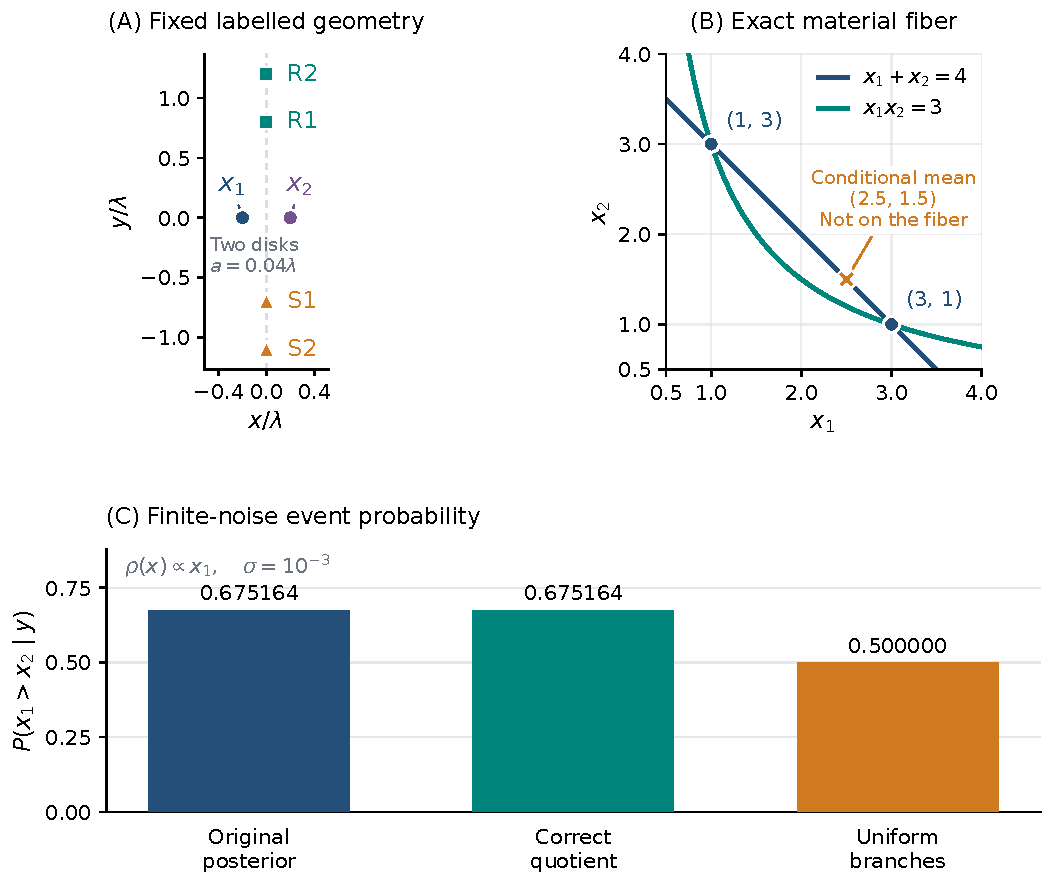
\includegraphics[width=\textwidth]{figures/two_cell_structure.pdf}
\caption{二单元 Maxwell 材料对称、可观测商与条件概率。（A）固定带标签的源、接收器及两圆盘材料几何。（B）$(1,3)$ 的精确材料纤维为 $x_1+x_2=4$ 与 $x_1x_2=3$ 的两个交点；在 $\rho\propto x_1$ 下，两支权重为 $1/4,3/4$，条件均值 $(2.5,1.5)$ 本身不在纤维上。（C）有限噪声下，原材料积分和正确商积分给出相同事件概率，均匀分支控制错误。面板 B 的精确纤维条件概率与面板 C 的带噪 posterior 是两个不同对象。}
\end{figure}
\clearpage

\subsection{输入、输出与独立合同}

附带的 \texttt{CODEX\_PROTOCOL\_ZH.txt} 是可直接交给 Codex 的完整执行协议。本节给出研究判断所需的紧凑版本。所有新实验在独立目录运行，R6/R7 的冻结报告、代码与账本只读。输入应包括：物理合同、原 prior、每个 decoder 的支持、源接收标签、Green 自项、噪声实化、任务定义、比较基线、种子与预算。

必须保存三类互不替代的证据：
\begin{enumerate}
\item \textbf{物理证据}：材料、全源电流、完整复预测、构成残差、被动性、prior 支持、resolvent 稳定性和独立复核。
\item \textbf{代数几何证据}：生成元恒等式/逆/组合、适用域、数值秩全谱、分支代表、连续参数、chart 转移、判别式事件及覆盖级别。
\item \textbf{概率与成本证据}：原测度、分支权重、coarea/恢复 Jacobian、参考积分、遗漏资格、失败尝试、全部分解与 RHS、CPU/wall time、内存。
\end{enumerate}

\subsection{E0--E4 的依赖顺序与成功门}

\begin{longtable}{p{.10\textwidth}p{.37\textwidth}p{.43\textwidth}}
\toprule 阶段 & 最小输入与测试 & 成功门与停止条件\\\midrule\endhead
E0 & $z^n$、圆、$a+b^2$、$V=QD$、三次映射、有限噪声链；明确 prior。 & 解析逆像、轨道、组合及概率对照均正确。错把 gauge 当材料或错权重时先停止修复。\\
E1 & 已完成两 cell 阳性；再用非对称 4--9 cell 真实 Green 模型。 & 完整物理验证；至少一个暗电流不可实现反例；扩展研究需真实不同材料或独立正则纤维依据。\\
E2 & 同一批材料及同一 prior；完整 Fourier/Wavelet、合法 Gaussian、材料 tangent、current chart。 & 往返材料保持，先验推前一致，支持变化单独标记。仅换基不算发现物理多解。\\
E3 & 从 E1 已有独立歧义证据的系统出发；比较 Full-J、multi-start、continuation、适用 CSI/SOM。 & 精确生成元须证闭合/逆/合法域；更强覆盖需限定域证书。只有端点或靠放松容差则降级。\\
E4 & 低维可信原空间积分；正确纤维、均匀轨道与错误边缘对照。 & 证据、均值、非线性任务、事件、branch mass 全部匹配；否则只能称几何枚举。\\\bottomrule
\end{longtable}

\textbf{推荐下一项最小问题}：一个非对称 4--9 cell TM 系统，预先固定全部标签，选择合法实材料内点和明确的新 prior。先构造 $n>k$ 的小型子问题，以常秩与 $n-r>0$ 作为精确局部纤维存在的独立依据；再比较共享材料 current chart 与直接材料隐函数/Full-J chart 对同一连通纤维的合法覆盖和条件积分费用。这里的目标不是发现维数计数已保证的 null，而是检验图册是否\emph{更可计算}。

另设 $n\le k$ 或满列秩子问题寻找远处分支，允许结果为没有发现。不要在看到结果后删 receiver 来制造成功；如需不同采集，建立新 contract ID。原 Full66 的离散远分支问题与新完整材料的连续纤维问题应分别注册。

\subsection{预算、数值资格与比较阈值}

以下是后续\emph{建议预算}，不是本轮已经使用的费用：每 run 最多 10,000 个实际复线性 RHS、2 CPU 小时、8 GB 峰值内存；整轮 30,000 RHS 硬上限。CPU 按线程累计，wall time 另记。结构构建、失败路径与认证都计入，不通过另开 run 绕过总上限。

float64 初筛可预注册归一化状态残差与完整观测差均不超过 $10^{-10}$，但这只是浮点门槛。数学精确只来自恒等式、符号推导或严格区间证书。数值 rank 记录缩放、全部谱、阈值与独立导数检查；不得把 $10^{-8}$ 以下的值直接当作零。

有限噪声验收始终对同一个 $y$，使用声明的 covariance 和 likelihood；噪声球可按预定 Gaussian 分位数选定，但仍不是等价类。路径相邻距离不能替代锚点检查。

E4 参考证据宜达到 $10^{-6}$ 或更好的数值精度；两种正确算法的证据相对差不超过 $\max(10^{-4},10\times\text{参考误差})$，归一化材料均值误差不超过 $10^{-4}$，事件/分支概率误差不超过 $10^{-3}$。Monte Carlo 则用预注册置信区间和 ESS。参考不够准时结论是参考不足，不事后放宽门槛。

效率门可预注册为相同覆盖与任务误差下总成本改善至少 $20\%$，并报告全部重复结果；这只是首轮决策阈值，不是统计显著性定理。小系统时间若由解释器或内存开销主导，不应外推为 Maxwell 大规模加速。

\subsection{后续三种决策}

\textbf{STOP}：只有非法暗电流；跨表示只是重复材料；exact 声明依赖放宽容差；原 prior 被换掉；缺乏比普通 corrector/continuation 更好的覆盖或费用；或者预算到限。停止对应研究主张，保留所有负面证据。

\textbf{CONDITIONAL GO}：有合法的非对称材料纤维/分支，或有独立覆盖证书，但正确概率或费用收益仍缺一项。下一轮只解决明确缺口。

\textbf{GO}：非对称小型 Maxwell 中获得可核验的更好分支覆盖、可计算图册或净物理费用收益，E4 正确测度通过，并与最强适用基线比较成立。之后才设计 Full66 或完整 576 实材料实验，二者继续分开。

\section{七个命题的答案与论文原创性判断}

\subsection{七个问题的条件答案}

\begin{longtable}{p{.08\textwidth}p{.25\textwidth}p{.57\textwidth}}
\toprule 命题 & 结论 & 关键条件或反例\\\midrule\endhead
1 & 简单群只在额外结构下完整刻画纤维。 & 集合层总有巨大置换群；光滑作用需等秩、等响应像，完整轨道需齐性/主丛等结构。三次实映射与自交浸入反例否定通用简单群。\\
2 & 跨 decoder 图册应先除 gauge，关系 decoder 用关联状态。 & submersion 可取局部 section；不同维数可同材料，非单射过渡一般不可逆。严格保材料循环不产生新世界。\\
3 & 常秩局部纤维维数为 $d-r$，满列秩局部单射。 & 不排除远处离散逆解。两 cell Maxwell 同时有 rank 2 与两个分支；Full66 rank66 不支持局部连续群。\\
4 & 有限噪声邻接不传递，也不构成等价群。 & 固定锚点、likelihood、log-ratio/TV 界与遗漏质量分开处理；近邻连通分量不是物理纤维。\\
5 & 可只反演商并复用 prior 核，当且仅当 likelihood 因子化。 & 标准 Borel disintegration；Gaussian 全数据族对应 forward 因子化；单点 quotient 不能替代带噪 quotient posterior。\\
6 & 有限固定生成元不能逐点列举连续纤维。 & 连续流族在同一正则连通分量上有条件覆盖；其他分量/strata 需额外箭头与证书；monodromy 需有限覆盖。\\
7 & 成本收益有条件，不能由代数名称保证。 & 已知对称可复用预测；current lift 可能膨胀，精确轨道质量可含 permanent；要比较冷启动总成本与任务误差。\\\bottomrule
\end{longtable}

\subsection{哪些内容已经属于成熟数学或既有电磁方法}

关系群胚、常秩/轨道定理、紧群不变量、覆盖 monodromy、disintegration/coarea、MH、Rao--Blackwell、LIS 以及数值代数几何都不能作为本研究独立首创。Maxwell 非辐射源、转换光学张量等价和 CSI/SOM 状态 lifting 也已有对应研究。

特别值得警惕的是两条重叠：一是把 Maxwell 离散状态写成多项式并用 homotopy 找根，并非新的研究概念；Everett 1996 已在小 Helmholtz 逆问题中实际枚举正实根，Vasco 2000 进一步研究代数化和消元。[R12,R13] 二是 current 的确定/模糊分解和材料显式更新已有 CSI/TSOM 前例。[R10,R11] 本轮二单元推导适合作为可审计的验证基准，尚不足以构成强 TAP 的核心贡献。

\textbf{近期直接先例。} Everett 于 2026-10-09 在线发表的研究，已对一维/二维电磁扩散的离散材料多项式系统，使用周期辅助参数和 Euler--Newton 路径寻找同数据的多个根，并区分正、负电导率候选。[R22] 因而 ``电磁逆问题多项式化后从一个解追踪其他解'' 也不能作为 Z-ALG 首创。

对这类方法的数学解释仍须独立审核：根集不自动成为循环群；往返线段在唯一正则提升下没有非平凡 monodromy，前文已经给出证明及奇异例外。$N$ 个方程、$N$ 个未知量也不意味着至多 $N$ 个根，反例 $x_i^2-1=0$ 有 $2^N$ 个非奇异根；一般零维多项式系统需采用正确的次数或稀疏根数界。新论文提供的有价值候选发现应与这些未成立的一般推断区分。

后续 E3 的普通 continuation 基线应包含适用于同一问题的此类周期参数跟踪，并保存奇异事件和跳支。不能因为路径法有合格端点就赋予它全覆盖、物理可行路径或 posterior 权重；同样不能因为其全局解释不足便忽略其实际搜索价值。

\subsection{最有希望的论文贡献：依次排序}

\textbf{第一优先：材料一致性与可认证纤维图册。} 在真实、非对称、多源 Maxwell 子问题中，把接收器暗空间缩为可实现材料图册；给出节点、被动性、prior 支持和 resolvent 的完整处理，并在有界材料域上证明或严格认证比基线更多的分支/分量。独立价值来自材料覆盖，不来自联立方程本身。

\textbf{第二优先：正确概率的可计算分支/纤维积分。} 在相同原 prior 下实现条件核、图册去重和任务积分，证明误差或遗漏界，并以相同费用展示对材料事件和风险的改善。这里的创新应是 Maxwell 特有的可计算分解或证书，而非重新证明通用 Bayes 分解。

\textbf{第三优先：新的合法材料变换或实验设计结论。} 若能在普通标量、固定磁导率的合理采集下发现非显然的精确变换，给出明确条件、覆盖和费用，可能构成独立理论论文。现有两 cell 镜像交换太简单，只能作为阳性例子；全各向异性坐标变换则已有文献，不宜包装成新结论。

\textbf{第四优先：有条件的 quotient imaging 加速。} 必须表明 quotient prior、likelihood 和条件生成器整体比直接反演便宜，且任务误差/覆盖相同。若只是把 $F(m)$ 命名为 $u$，然后在每个 $u$ 重新求一次原逆问题，则没有算法贡献。

\subsection{对强 IEEE TAP 的现实判断}

以目前结果直接写成 ``群胚统一 Maxwell 多解''，发表价值不足；抽象统一与几个 toy 不会消除与既有理论的重叠。以目前结果组织一份严谨研究设计和可复现实验基准，则是有价值的起点。

若后续取得非对称、多源物理模型上的新覆盖证书、材料有效的低费用生成器，或正确概率积分的任务收益，并展示适度网格/多频验证及离散误差影响，可以形成独立 Maxwell 方法论文。若主体贡献更偏代数复杂性、奇异测度或一般分层定理，数学反问题或计算数学期刊也可能更匹配；不能用 TAP 标签替代实际电磁增量。

本轮建议为\textbf{CONDITIONAL GO：建立 Research Z-ALG，但先以材料约束和正确测度为主线}。最小下一问题已经明确：在一个非对称小型 TM 系统的已知正维正则纤维上，比较 current 图册与直接材料 continuation 的合法覆盖、条件积分和总成本。若这一关没有优势，应停止扩大 ``通用代数探索''；若成功，再分别研究离散远分支和原 Full66 适用性。

用户提出的愿景在数学上可实现的精确形式是
\begin{equation}
y\longmapsto\nu^y(du),\qquad
(u,\xi)\longmapsto M\sim K(\cdot\mid u),
\end{equation}
其中 $\xi$ 包含分支和连续纤维随机性，$K$ 严格来源于原材料 prior。最大的开放问题并不是这个分解是否存在，而是\textbf{能否对具体 Maxwell 合同把它构造得比直接后验计算更完整、更稳定或更便宜}。

\newpage
\section{文献、输入来源与可复现附件}

\subsection{文献核查说明}

以下优先使用原论文、作者机构、原出版社与官方软件文档。检索截止日为 2026 年 10 月 29 日。文献支持所标明的既有事实；本报告的条件推导和反例另给证明，不把标准理论或未完成实验包装为原创定理。公开信息检索不等于穷尽全部文献，正式投稿前仍需针对最终具体贡献更新最接近方法的对照。

\begin{enumerate}[label={[R\arabic*]},leftmargin=3.1em,itemsep=7pt]
\item J. M. Lee, \emph{Introduction to Smooth Manifolds}, 2nd ed., Springer, 2013, Chapter 4. 常秩、浸入、submersion 和局部逆。\href{https://link.springer.com/chapter/10.1007/978-1-4419-9982-5_4}{出版社章节}。
\item H. J. Sussmann, ``Orbits of Families of Vector Fields and Integrability of Distributions,'' \emph{Transactions of the AMS}, 180, 171--188, 1973. \href{https://doi.org/10.1090/S0002-9947-1973-0321133-2}{DOI: 10.1090/S0002-9947-1973-0321133-2}。
\item A. S. Bandeira et al., ``Estimation under group actions: recovering orbits from invariants,'' \emph{Applied and Computational Harmonic Analysis}, 66, 236--319, 2023; preprint 2017. \href{https://arxiv.org/abs/1712.10163}{arXiv:1712.10163}。已指定群的 orbit recovery，与发现 Maxwell 对称不同。
\item G. W. Schwarz, ``Smooth functions invariant under the action of a compact Lie group,'' \emph{Topology}, 14, 63--68, 1975. \href{https://doi.org/10.1016/0040-9383(75)90036-1}{DOI: 10.1016/0040-9383(75)90036-1}。
\item S. Holman and V. Torega, ``Boundary Recovery of Anisotropic Electromagnetic Parameters for the Time Harmonic Maxwell's Equations,'' preprint 2023. \href{https://arxiv.org/abs/2303.06688}{arXiv:2303.06688}；\href{https://doi.org/10.1007/s12220-023-01499-0}{期刊 DOI}。支持各向异性参数的微分同胚 gauge 背景。
\item I. Androulidakis and G. Skandalis, ``The holonomy groupoid of a singular foliation,'' preprint 2006. \href{https://arxiv.org/abs/math/0612370}{arXiv:math/0612370}。奇异 foliation 的 groupoid 有明确向量场模条件。
\item A. Hatcher, \emph{Algebraic Topology}, Section 1.3. \href{https://pi.math.cornell.edu/~hatcher/AT/AT.pdf}{作者公开全文}。覆盖、路径提升与 monodromy。
\item P. Breiding and S. Timme, ``HomotopyContinuation.jl: A Package for Homotopy Continuation in Julia,'' \href{https://arxiv.org/abs/1711.10911}{arXiv:1711.10911}；\href{https://www.juliahomotopycontinuation.org/HomotopyContinuation.jl/stable/monodromy/}{官方 monodromy 文档}。文档包含群作用复用及数值验证限制。
\item J. D. Hauenstein and F. Sottile, ``Algorithm 921: alphaCertified: Certifying Solutions to Polynomial Systems,'' \emph{ACM Transactions on Mathematical Software}, 2012. \href{https://doi.org/10.1145/2331130.2331136}{DOI: 10.1145/2331130.2331136}。单根认证不等于根集完整性。
\item P. M. van den Berg and R. E. Kleinman, ``A contrast source inversion method,'' \emph{Inverse Problems}, 13, 1607--1620, 1997. \href{https://doi.org/10.1088/0266-5611/13/6/013}{DOI: 10.1088/0266-5611/13/6/013}。
\item X. Chen, Y. Zhong and K. Agarwal, ``Subspace methods for solving electromagnetic inverse scattering problems,'' \emph{Methods and Applications of Analysis}, 17(4), 407--432, 2010. \href{https://archive.intlpress.com/site/pub/files/_fulltext/journals/maa/2010/0017/0004/MAA-2010-0017-0004-a006.pdf}{原出版社全文}。确定/模糊电流、SOM、TSOM 和相关 Fourier 加速。
\item M. E. Everett, ``Homotopy, Polynomial Equations, Gross Boundary Data, and Small Helmholtz Systems,'' \emph{Journal of Computational Physics}, 124(2), 431--441, 1996. \href{https://doi.org/10.1006/jcph.1996.0070}{DOI: 10.1006/jcph.1996.0070}。小型离散 Helmholtz 的多根枚举先例。
\item D. W. Vasco, ``An algebraic formulation of geophysical inverse problems,'' \emph{Geophysical Journal International}, 142(3), 970--990, 2000. \href{https://doi.org/10.1046/j.1365-246x.2000.00188.x}{DOI: 10.1046/j.1365-246x.2000.00188.x}。
\item P. Li and J. Wang, ``Nonradiating sources of Maxwell's equations,'' 2024. \href{https://arxiv.org/abs/2402.10407}{arXiv:2402.10407}。源的非唯一性不直接给共同材料可实现性。
\item P. Diaconis, S. Holmes and M. Shahshahani, ``Sampling From A Manifold,'' 2012. \href{https://arxiv.org/abs/1206.6913}{arXiv:1206.6913}。coarea 条件密度与流形采样。
\item J. T. Chang and D. Pollard, ``Conditioning as disintegration,'' \emph{Statistica Neerlandica}, 51(3), 287--317, 1997. \href{https://doi.org/10.1111/1467-9574.00056}{DOI: 10.1111/1467-9574.00056}。
\item T. Cui et al., ``Likelihood-informed dimension reduction for nonlinear inverse problems,'' 2014. \href{https://arxiv.org/abs/1403.4680}{arXiv:1403.4680}。统计重要方向与精确观测商的区别。
\item O. Zahm et al., ``Certified dimension reduction in nonlinear Bayesian inverse problems,'' \emph{Mathematics of Computation}, 91, 1789--1835, 2022.\newline \href{https://arxiv.org/abs/1807.03712}{arXiv:1807.03712}。条件 likelihood profile 与认证误差条件。
\item A. Spantini et al., ``Goal-oriented optimal approximations of Bayesian linear inverse problems,'' 2017. \href{https://arxiv.org/abs/1607.01881}{arXiv:1607.01881}。任务降维的线性 Gaussian 基线。
\item L. G. Valiant, ``The Complexity of Computing the Permanent,'' \emph{Theoretical Computer Science}, 8, 189--201, 1979. \href{https://doi.org/10.1016/0304-3975(79)90044-6}{DOI: 10.1016/0304-3975(79)90044-6}。
\item M. Jerrum, A. Sinclair and E. Vigoda, ``A polynomial-time approximation algorithm for the permanent of a matrix with nonnegative entries,'' \emph{JACM}, 51(4), 671--697, 2004. \href{https://www.inf.ed.ac.uk/publications/report/0460.html}{作者机构报告}。精确困难不排除有误差保证的随机近似。
\item M. E. Everett, ``Multiple solutions to geophysical inverse problems via tracking flights across a deeply incised model landscape,'' \emph{Geophysical Journal International}, 247(3), ggag432, online 2026-10-09. \href{https://doi.org/10.1093/gji/ggag432}{DOI: 10.1093/gji/ggag432}。近期直接相关的电磁扩散多项式路径搜索先例；本文不采纳一般根集自动为循环群的推断。
\end{enumerate}

\subsection{既有科研材料的读取范围}

\textbf{[I1] Research P3L-R6。} 公共仓库 \texttt{migodam/b1-probabilistic-maxwell-imaging}，科学版本前缀 \texttt{d1bdc8aceae4c}。实际读取主报告、理论与反例、分层概率和 Track A copula 报告。\href{https://raw.githubusercontent.com/migodam/b1-probabilistic-maxwell-imaging/d1bdc8aceae4cd6a843f873b61b019d5eee3cd1d/research/p3l_r6_task_optimal_maxwell/RESEARCH_REPORT_ZH.md}{冻结主报告}；完整文件名和路径见附件 manifest。

\textbf{[I2] Research P3L-R7。} 同仓库，读取快照前缀 \texttt{975ebe7f17c2}；这标识本次读取快照，不声称它是 R7 最初发布的 freeze commit。实际读取 START\_HERE、主报告、E1 gauge audit、E2 材料纤维结果、理论、资源账本与 Go/No-Go。\href{https://raw.githubusercontent.com/migodam/b1-probabilistic-maxwell-imaging/975ebe7f17c2ba837a8cac0a5f8eb4ccf7d4e19b/research/p3l_r7_material_solution_fibers/RESEARCH_REPORT_ZH.md}{读取快照主报告}。

\textbf{[I3] 原 Research Z。} 包名为\newline
\path{Research_Z_Physics_Context_Latent_Generative_Maxwell_Imaging.zip}，2026-10-15 理论设计包。本次读取主报告、理论说明、claim ledger 与 README；完整实材料 576 维在主报告 3.A，$8\times32$ 采集在第 9 节。此包没有新的训练或 posterior 实验。

\textbf{[I4] TSOM 及其他先前结论。} SOM/TSOM 的原作者论文 [R11] 已核查。PairTSOM、F/F3 的特定项目实验在本报告中作为用户明确提供、并与已读后续报告相容的研究约束；不宣称已独立复现或完整读到其全部原始实验包。R7-T/R8-T 相关理论 PDF 已检查引用段落，其理论讨论不作为 R7 实验新增证据。

附件的 \texttt{SOURCE\_MANIFEST.json} 保存 R6/R7 完整 commit、来源路径与字节数；最终附件 manifest 再记录本次全部交付文件的 SHA256。原历史大型实验在本轮未重跑。

\subsection{可复现附件内容}

研究包包括：本报告的 LaTeX 源码；可直接执行的中文 Codex 协议；解析/monodromy toy 脚本及结果；真实二单元 TM/VIE 脚本及完整 JSON；带噪 E4 双积分脚本及结果；来源与校验 manifest；重建说明。

字体文件来自 Noto CJK 官方仓库；重建说明给出下载地址和 XeLaTeX 命令。附件不捆绑既有项目仓库或训练数据，也不修改旧轮次记录。报告 PDF 是完整科研交付，源码和结果文件用于审计与后续复现。

\end{document}
